%!TEX program = xelatex
\documentclass{beamer}
%\documentclass[aspectratio=169]{beamer} %如果需要16:9
\usepackage{ctex}
\usepackage{times}
\usepackage{multicol}
\usepackage{multirow}
\usetheme{Warsaw}
\usepackage{tikz}
\usetikzlibrary{arrows,shapes,chains}
\usepackage[super,square]{natbib}
\usepackage{tabularx}
\usepackage{booktabs}
\usepackage{longtable}
\usepackage{graphicx}
%\usecolortheme{beaver}     % use white-grey colour style
%\beamersetaveragebackground{black!10}
% This is only inserted into the PDF information catalog. Can be left out.
\subject{presentation}
\keywords{example}
\useinnertheme{circles}%{rectangles}
\setbeamertemplate{itemize item}{$\circledast$}%{\checkmark}

%% ======================================================
%%     preamble
%% ======================================================
\title{基于SpringMVC架构WEB应用系统优化研究}
\author{答辩人:武斌}
\institute
{
  导师:郑海永\\
  电子系~中国海洋大学
  \and
   Department electronic engineering \\
  Ocean University Of China
}
% \date{\today}
\date{2017年5月25日}

\logo{
\includegraphics[height=0.09\textwidth]{./logo/Ocean_University_of_China.png}}


%% ======================================================
\begin{document}

%% ++++++++++++++++++++++++++++++++++++++++++++++++++++++
%% title page
%% ++++++++++++++++++++++++++++++++++++++++++++++++++++++
\begin{frame}
  \titlepage
\end{frame}

%% ++++++++++++++++++++++++++++++++++++++++++++++++++++++
%%     Table of Contents
%% ++++++++++++++++++++++++++++++++++++++++++++++++++++++
%\begin{frame}
    %\frametitle{Contents}
    %\tableofcontents
    %% 显示1-4section,不显示subsection
    %\tableofcontents[hidesubsections,sections={<1-4>}]
%\end{frame}

%% ++++++++++++++++++++++++++++++++++++++++++++++++++++++
%%     目录
%% ++++++++++++++++++++++++++++++++++++++++++++++++++++++
%\section{概述}
\begin{frame}
  \frametitle{目录}
  \begin{enumerate}
    \item<1-> 题目来源及目的
    \item<1-> 研究方法及内容
    \item<1-> 研究结论及展望
  \end{enumerate}
\end{frame}


%% ++++++++++++++++++++++++++++++++++++++++++++++++++++++
%%      正文
%% ++++++++++++++++++++++++++++++++++++++++++++++++++++++
%% ++++++++++++++++++++++++++++++++++++++++++++++++++++++
%%      选题背景
%% ++++++++++++++++++++++++++++++++++++++++++++++++++++++
%\section{选题来源和背景分析 }
%\subsection{系统结构}
\begin{frame}
  \frametitle{来源及目的}
  \begin{block}{题目来源}
  	\begin{itemize}
  		\item 本人在海信参与的项目,负责DevOps的研究和实践,目的是实现产品的持续交付和快速部署。
  		% \item 目前的参考文献中很少有针对于单一系统的整体性优化策略研究;
  	\end{itemize}
  \end{block}
  \begin{block}{研究目的}
  	\begin{itemize}
  		\item 研究系统开发过程中的代码交付、持续集成、服务器运维等方面的优化策略
      \item 基于现有的WEB项目研究一种切实可用的WEB平台开发运维优化方案,为有相同需求的研发人员提供借鉴和参考
  	\end{itemize}
  \end{block}
\end{frame}
%% ++++++++++++++++++++++++++++++++++++++++++++++++++++++
%%      研究内容
%% ++++++++++++++++++++++++++++++++++++++++++++++++++++++
\begin{frame}
  \frametitle{方法及内容}
  \begin{enumerate}
    \item<1-> 研究的基本框架
    \item<1-> 应用性能优化
    \item<1-> 数据库性能优化
    \item<1-> 服务器稳定性优化
  \end{enumerate}
\end{frame}

\begin{frame}
  \frametitle{平台开发基本框架}
  \begin{figure}
  \centering
    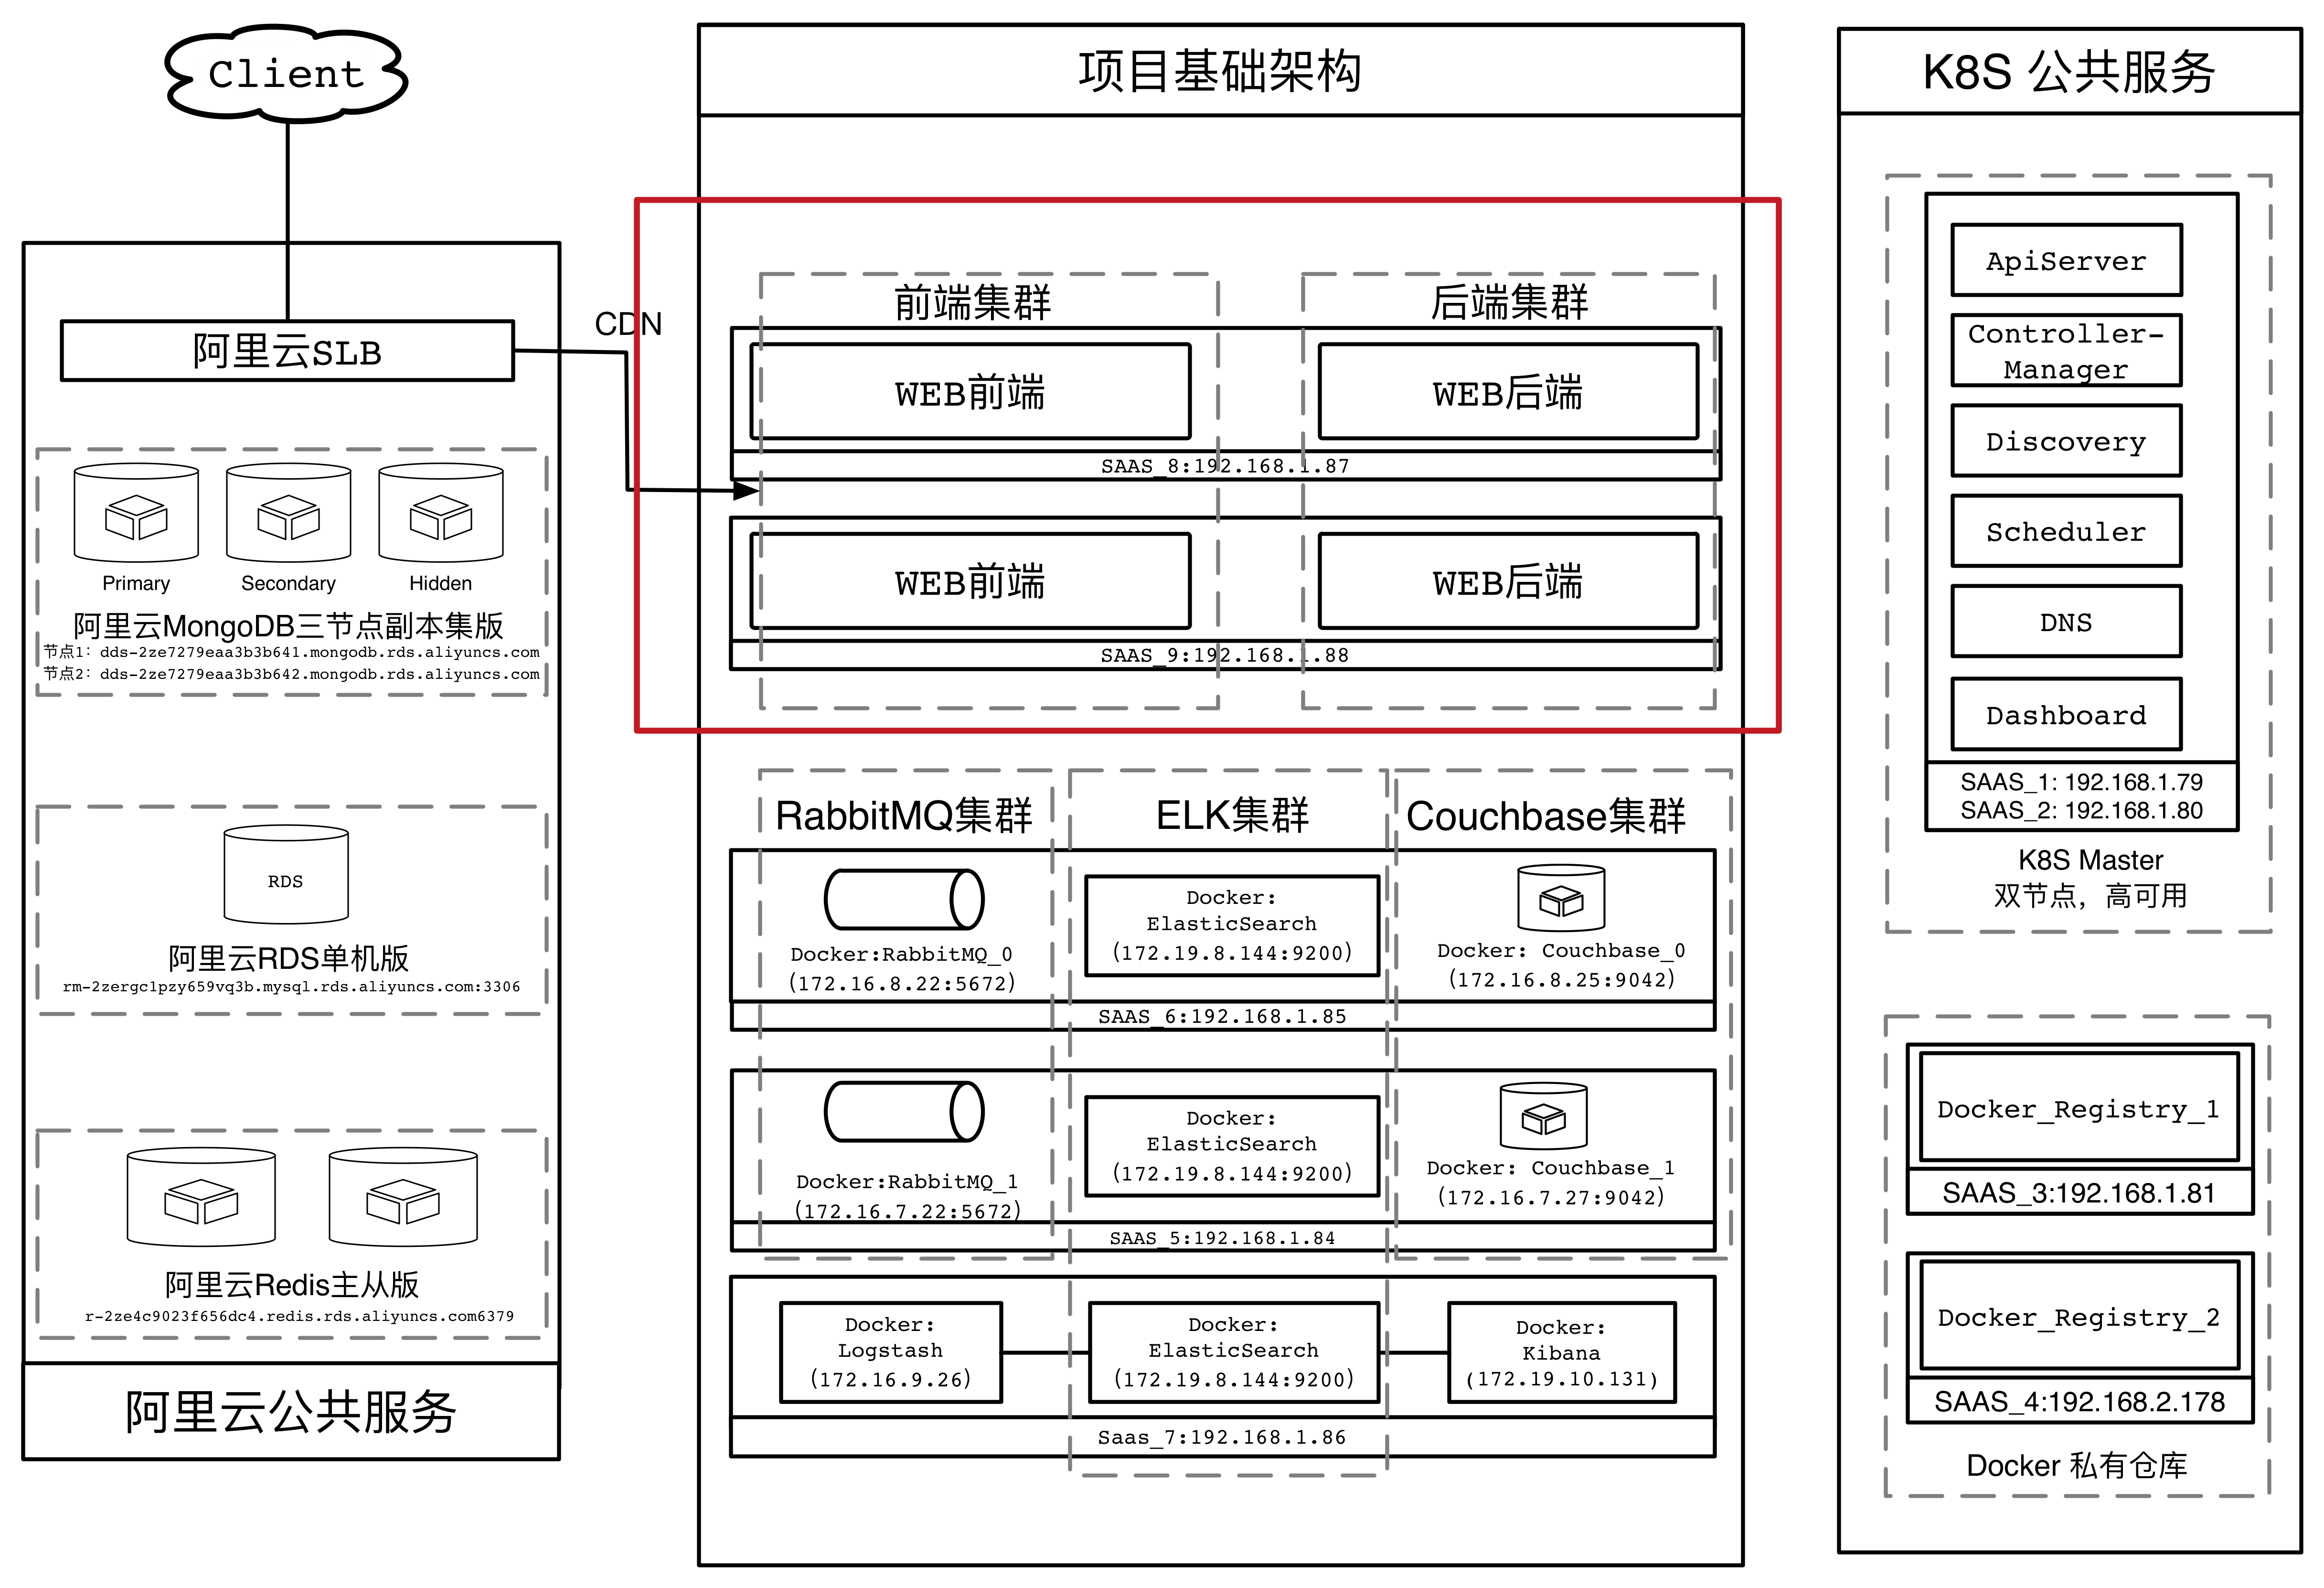
\includegraphics[width=\textwidth]{./img/02/deploy.png}
    % \caption{平台开发基本框架}
    \label{fig:deploy}
  \end{figure}
\end{frame}

\begin{frame}
  \frametitle{研究的主要内容}
  \begin{figure}
  \centering
    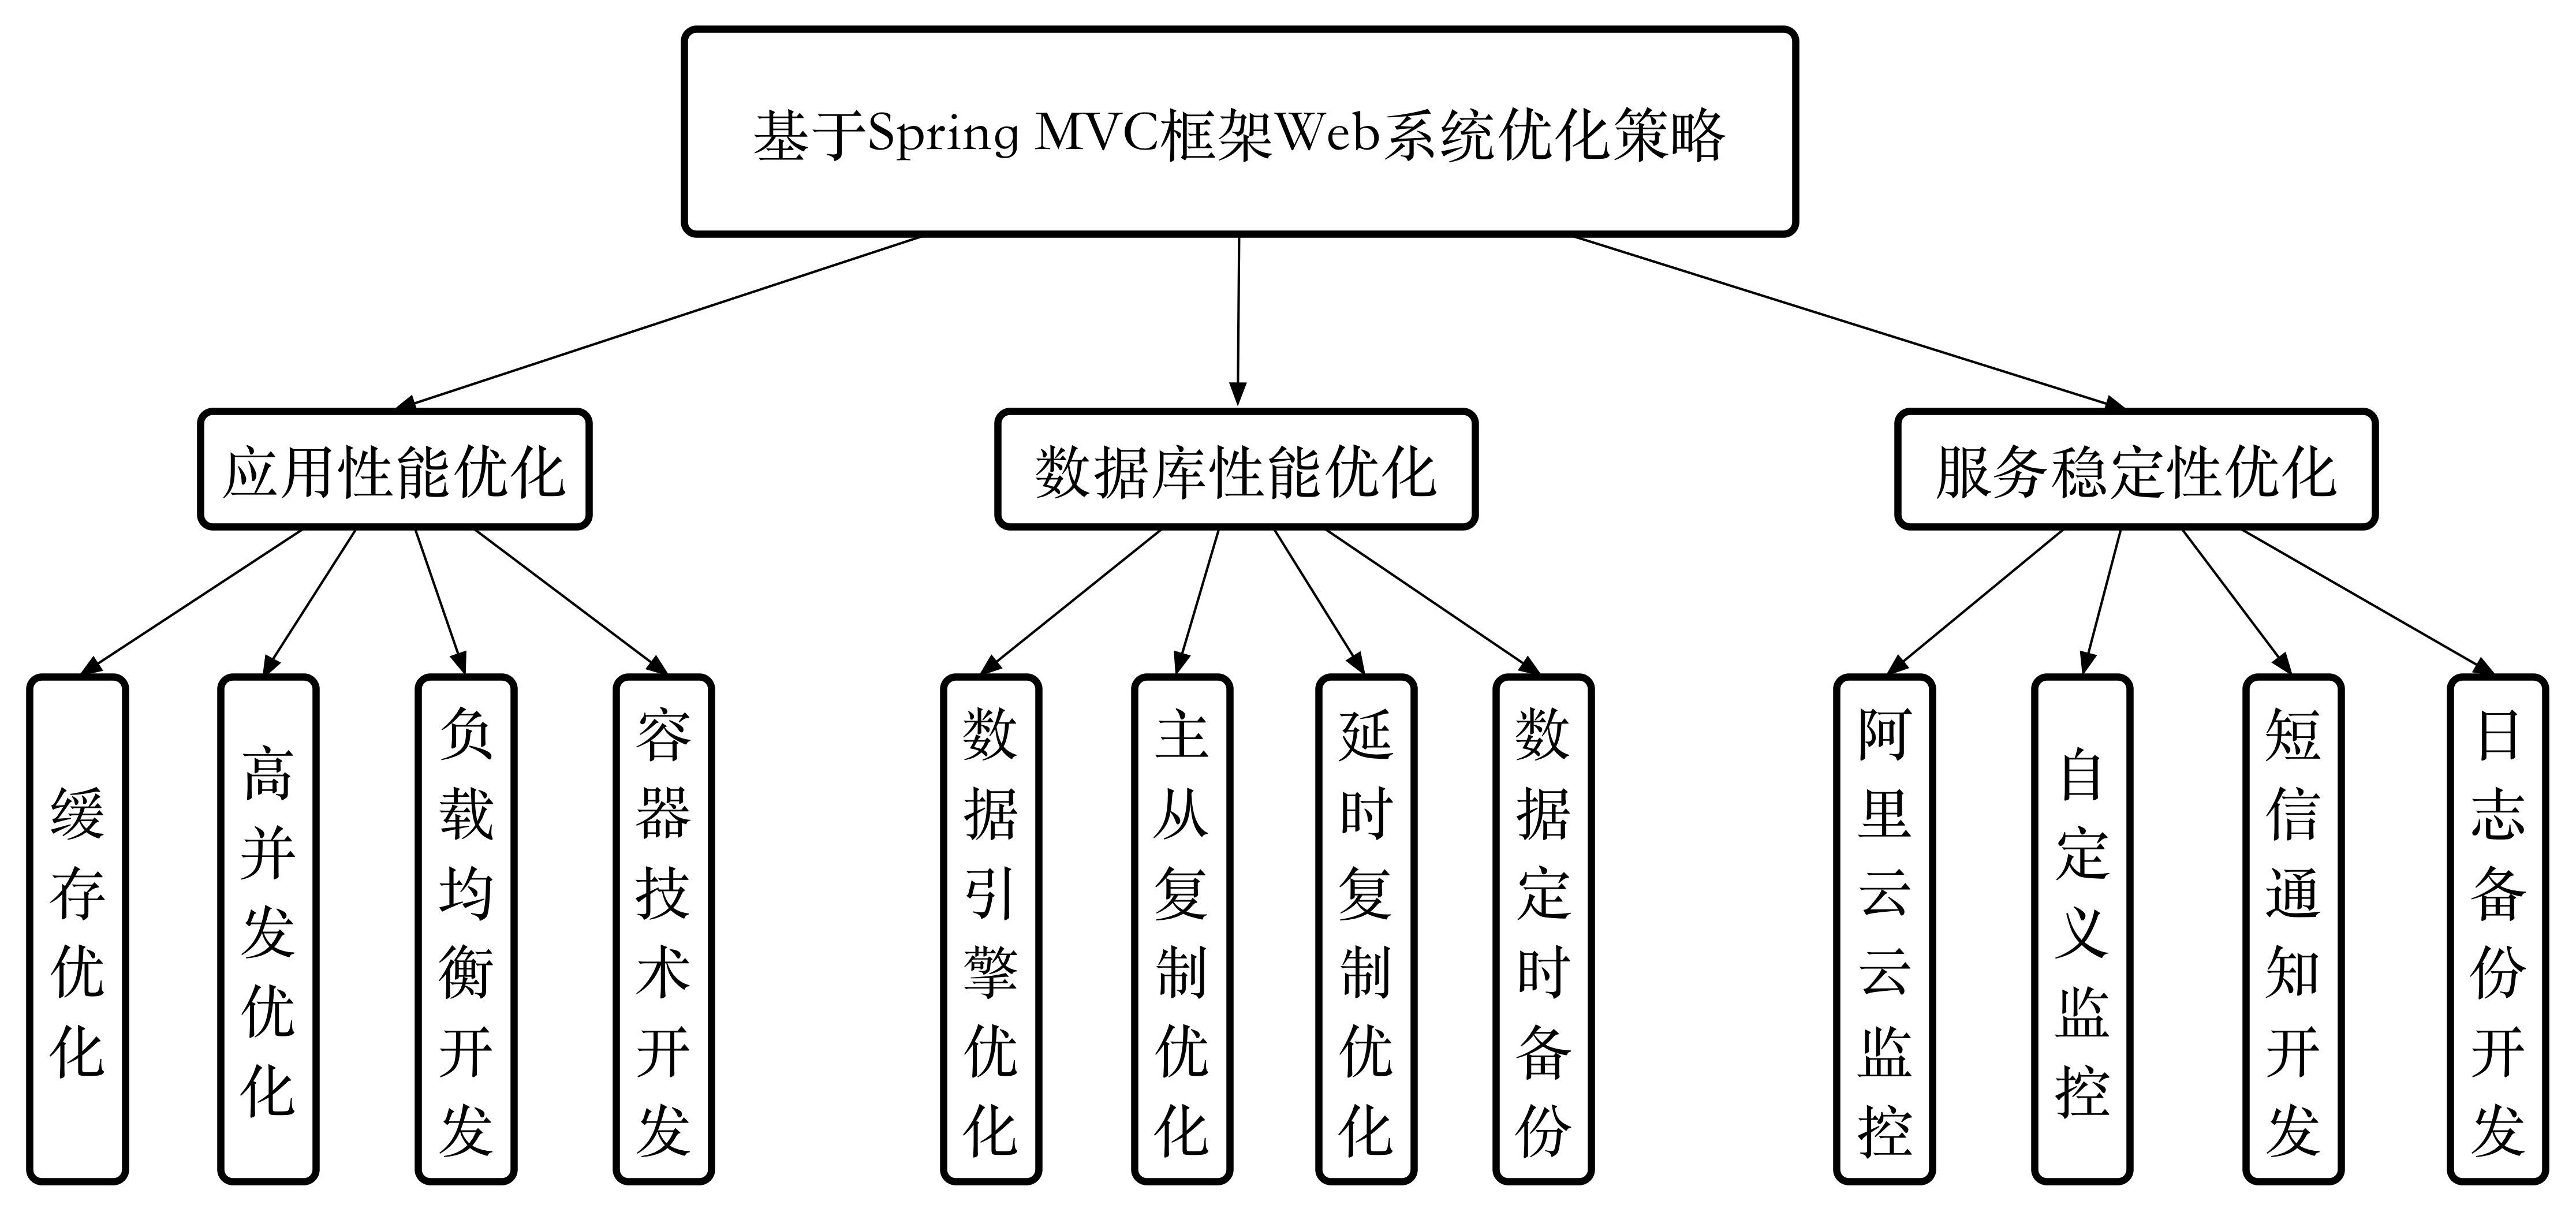
\includegraphics[height=5cm]{./img/02/summery.png}
    \caption{平台功能}
    \label{fig:summery}
  \end{figure}
\end{frame}

\begin{frame}
  \frametitle{一、应用性能优化}
    \begin{block}{1. Couchbase缓存优化}
      \begin{itemize}
        \item 将项目的基础数据在首次访问时加载到缓存中\cite{brown2013developing}
      \end{itemize}
    \end{block}
    \begin{columns}
      \begin{column}{0.40\textwidth}
        \rightline{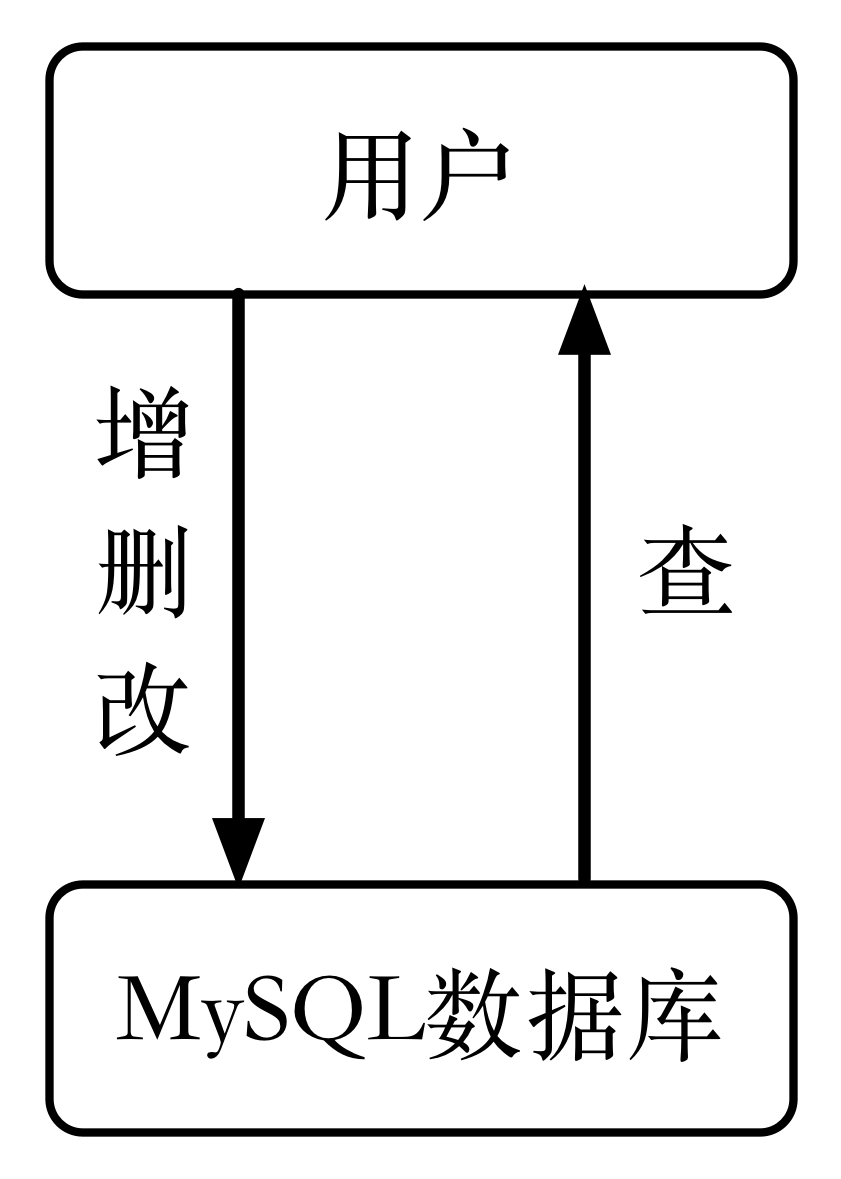
\includegraphics[height=3.5cm]{./img/02/couchbase1.png}}
      \end{column}
      \begin{column}{0.20\textwidth}
        \centering
        
\includegraphics[width=2cm]{./img/02/arrow.png}
        \label{fig:arrow}
      \end{column}
      \begin{column}{0.40\textwidth}
        \leftline{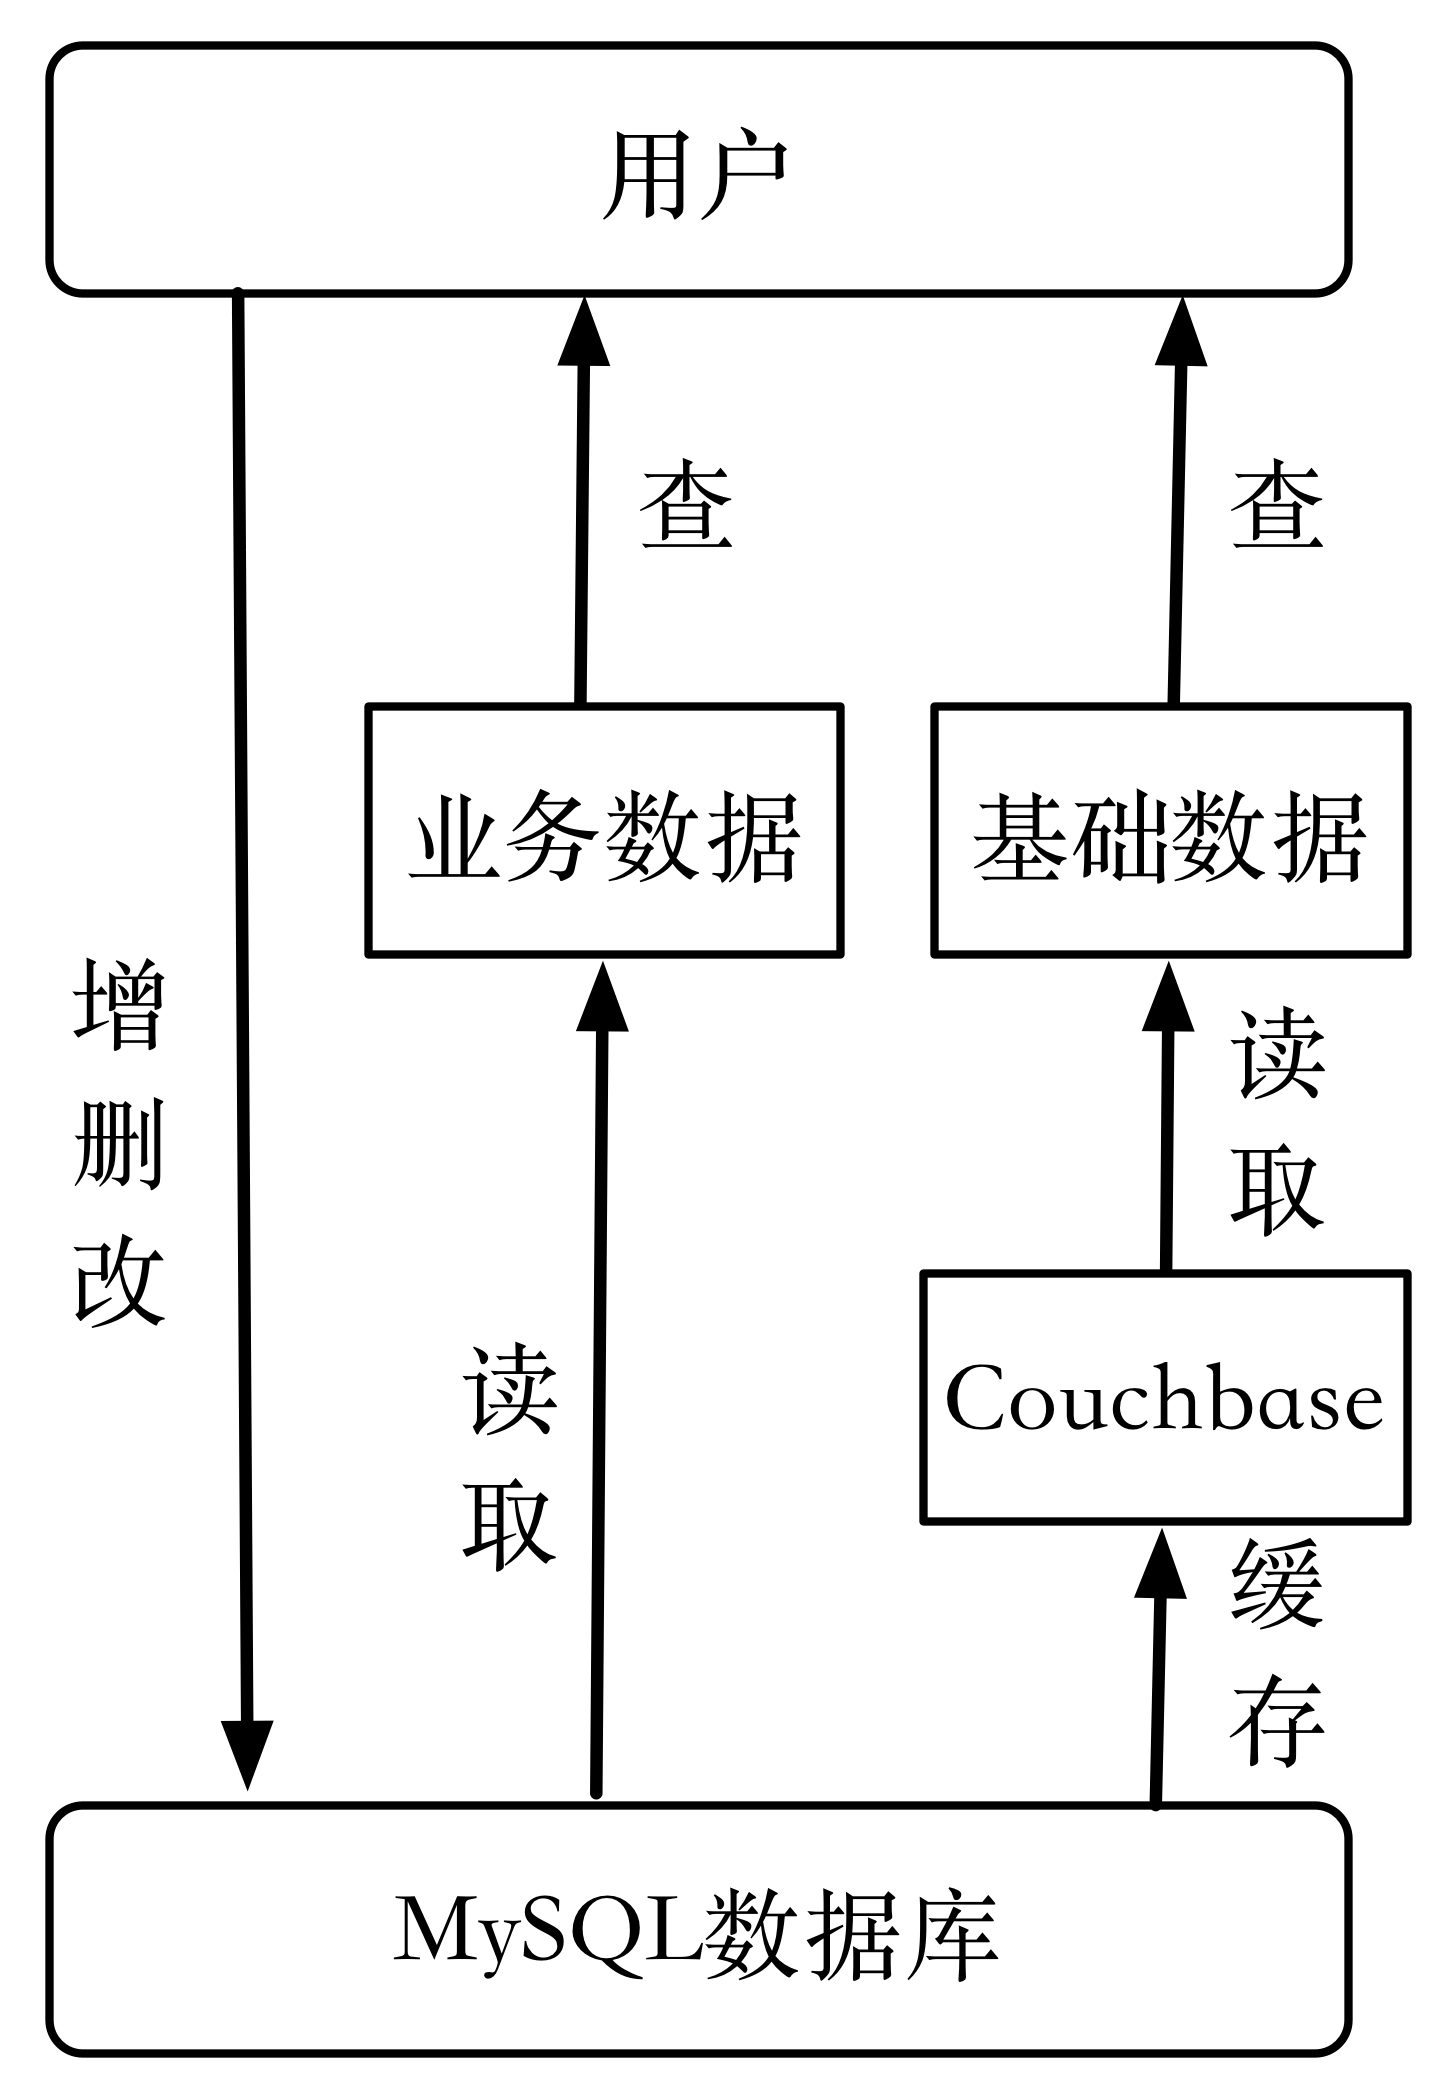
\includegraphics[height=3.5cm]{./img/02/couchbase2.png}}
      \end{column}
    \end{columns}
    \begin{table}[htb]
    \centering
    \begin{minipage}[t]{\linewidth} % 如果想在表格中使用脚注,minipage是个不错的办法
    \centering
    \scalebox{0.7}[0.7]{
    \label{tab:couchbase-test}
      \begin{tabularx}{\linewidth}{lXX}
        \toprule[1.5pt]
        {\heiti 测试参数} & {\heiti 关闭Couchbase} & {\heiti 开启Couchbase} \\\midrule[1pt]
        单次请求用时  &  0.670(s) & 0.113(s)\\
        请求失败次数 &  82 & 7 \\
        \bottomrule[1.5pt]
      \end{tabularx}
    }
    \end{minipage}
    \scalebox{0.7}[0.7]{\footnotesize{{ }{ }注: 10W次请求,每次100个并发}}
    \end{table}
\end{frame}


% \begin{frame}
%   \frametitle{一、应用性能优化}
%   \begin{table}[htb]
%   \centering
%   \begin{minipage}[t]{\linewidth} % 如果想在表格中使用脚注,minipage是个不错的办法
%   \caption[APR模式]{APR模式性能对比表}
%   \label{tab:couchbase-test}
%     \begin{tabularx}{\linewidth}{lXX}
%       \toprule[1.5pt]
%       {\heiti 测试参数} & {\heiti 关闭Couchbase} & {\heiti 开启Couchbase} \\\midrule[1pt]
%       单次请求用时  &  0.670(s) & 0.113(s)\\
%       请求失败次数 &  82 & 7 \\
%       \bottomrule[1.5pt]
%     \end{tabularx}
%   \end{minipage}
%   \end{table}
% 通过测试可以发现,开启Couchbase后系统的单次请求用时为0.113秒,而不使用Couchbase时单次请求用时为0.67秒,效率提升在83\%左右,这表示开启缓存后进行数据请求时,只需要耗费一次长时间的请求,数据建立缓存后获取效率将大大提升。除此之外,请求的失败次数也大大降低,这对于系统的稳定性来说提升特别明显。
% \end{frame}
\begin{frame}
  \frametitle{一、应用性能优化}
    \begin{block}{2. Tomcat高并发APR优化}
      \footnotesize{
      Tomcat 节约用户高并发的处理方式有NIO和APR两种方式\cite{蒋文旭2012大型高并发}:
      \begin{itemize}
        \item NIO 模式是一 个基于缓冲区、并能提供非阻塞 I/O 操作的 Java API
        \item APR模式是从操作系统级别解决异步IO问题,大幅度的提高服务器的处理和响应性能,是Tomcat 运行高并发应用的首选模式。
      \end{itemize}
      }
    \end{block}
    \begin{table}[htb]
      \centering
      \begin{minipage}[t]{0.8\linewidth} % 如果想在表格中使用脚注,minipage是个不错的办法
      \scalebox{0.85}[0.85]{
      \label{tab:tomcat-apr}
        \begin{tabularx}{\linewidth}{lXXX}
          \toprule[1.5pt]
          {\heiti 请求次数} & {\heiti 并发数量} & {\heiti APR模式} &  {\heiti NIO模式}\\
          \midrule[1pt]
          10000&10 &6612.60&8255.48\\
          50000  &  10 & 7480.96 & 8841.41 \\
          100000  &  10 & 6588.83 & 8355.85 \\
          10000  &  1000 & 6966.93 & 6155.21 \\
          50000  &  1000 & 9187.63 & 1957.35 \\
          100000  &  1000 & 7751.47 & - \\
          \bottomrule[1.5pt]
        \end{tabularx}
        }
      \end{minipage}
    \end{table}
\end{frame}
% \begin{frame}
%   \frametitle{一、应用性能优化}
%   低并发下,APR 模式同NIO 模式相比,吞吐量较低,但 相差不大;高并发下,APR 模式的优势明显,在 100000 次请求,每次并发 1000 个请求的情况下,NIO 模式无法 完成测试,通过数据可以看出,开启 APR 模式对于 WEB 平台应对高并发请求有 着非常重要的作用。
%   \begin{table}[htb]
%     \centering
%     \begin{minipage}[t]{0.8\linewidth} % 如果想在表格中使用脚注,minipage是个不错的办法
%     \caption[APR模式]{APR模式吞吐量对比表}
%     \scalebox{0.85}[0.85]{
%     \label{tab:tomcat-apr}
%       \begin{tabularx}{\linewidth}{lXXX}
%         \toprule[1.5pt]
%         {\heiti 请求次数} & {\heiti 并发数量} & {\heiti APR模式} &  {\heiti NIO模式}\\
%         \midrule[1pt]
%         10000&10 &6612.60&8255.48\\
%         50000  &  10 & 7480.96 & 8841.41 \\
%         100000  &  10 & 6588.83 & 8355.85 \\
%         10000  &  1000 & 6966.93 & 6155.21 \\
%         50000  &  1000 & 9187.63 & 1957.35 \\
%         100000  &  1000 & 7751.47 & - \\
%         \bottomrule[1.5pt]
%       \end{tabularx}
%       }
%     \end{minipage}
%   \end{table}
% \end{frame}
\begin{frame}
  \frametitle{一、应用性能优化}
    \begin{block}{3. 容器化开发部署优化优化}
      随着业务的扩展,目前一个WEB应用所使用的必要服务器数量已经扩展到了7个节点:
      \begin{enumerate}
        \item 应用服务节点*2
        \item 数据库节点*2
        \item ELK日志服务及其他服务节点*3
      \end{enumerate}
      如何快速部署一个新的服务节点必然是运维人员在新增节点时必须要面对的问题\cite{fink2014docker}。

      容器化是解决快速部署新节点和持续交付新服务的最优解决方案,他避免了每次安装软件的繁琐操作也节省了配置新的服务的各种配置成本。通过容器化,能够使开发运维的成本降低40\%以上。
    \end{block}
\end{frame}
\begin{frame}
  \frametitle{一、应用性能优化}
  \begin{columns}
    \begin{column}{0.50\textwidth}
      \centering
      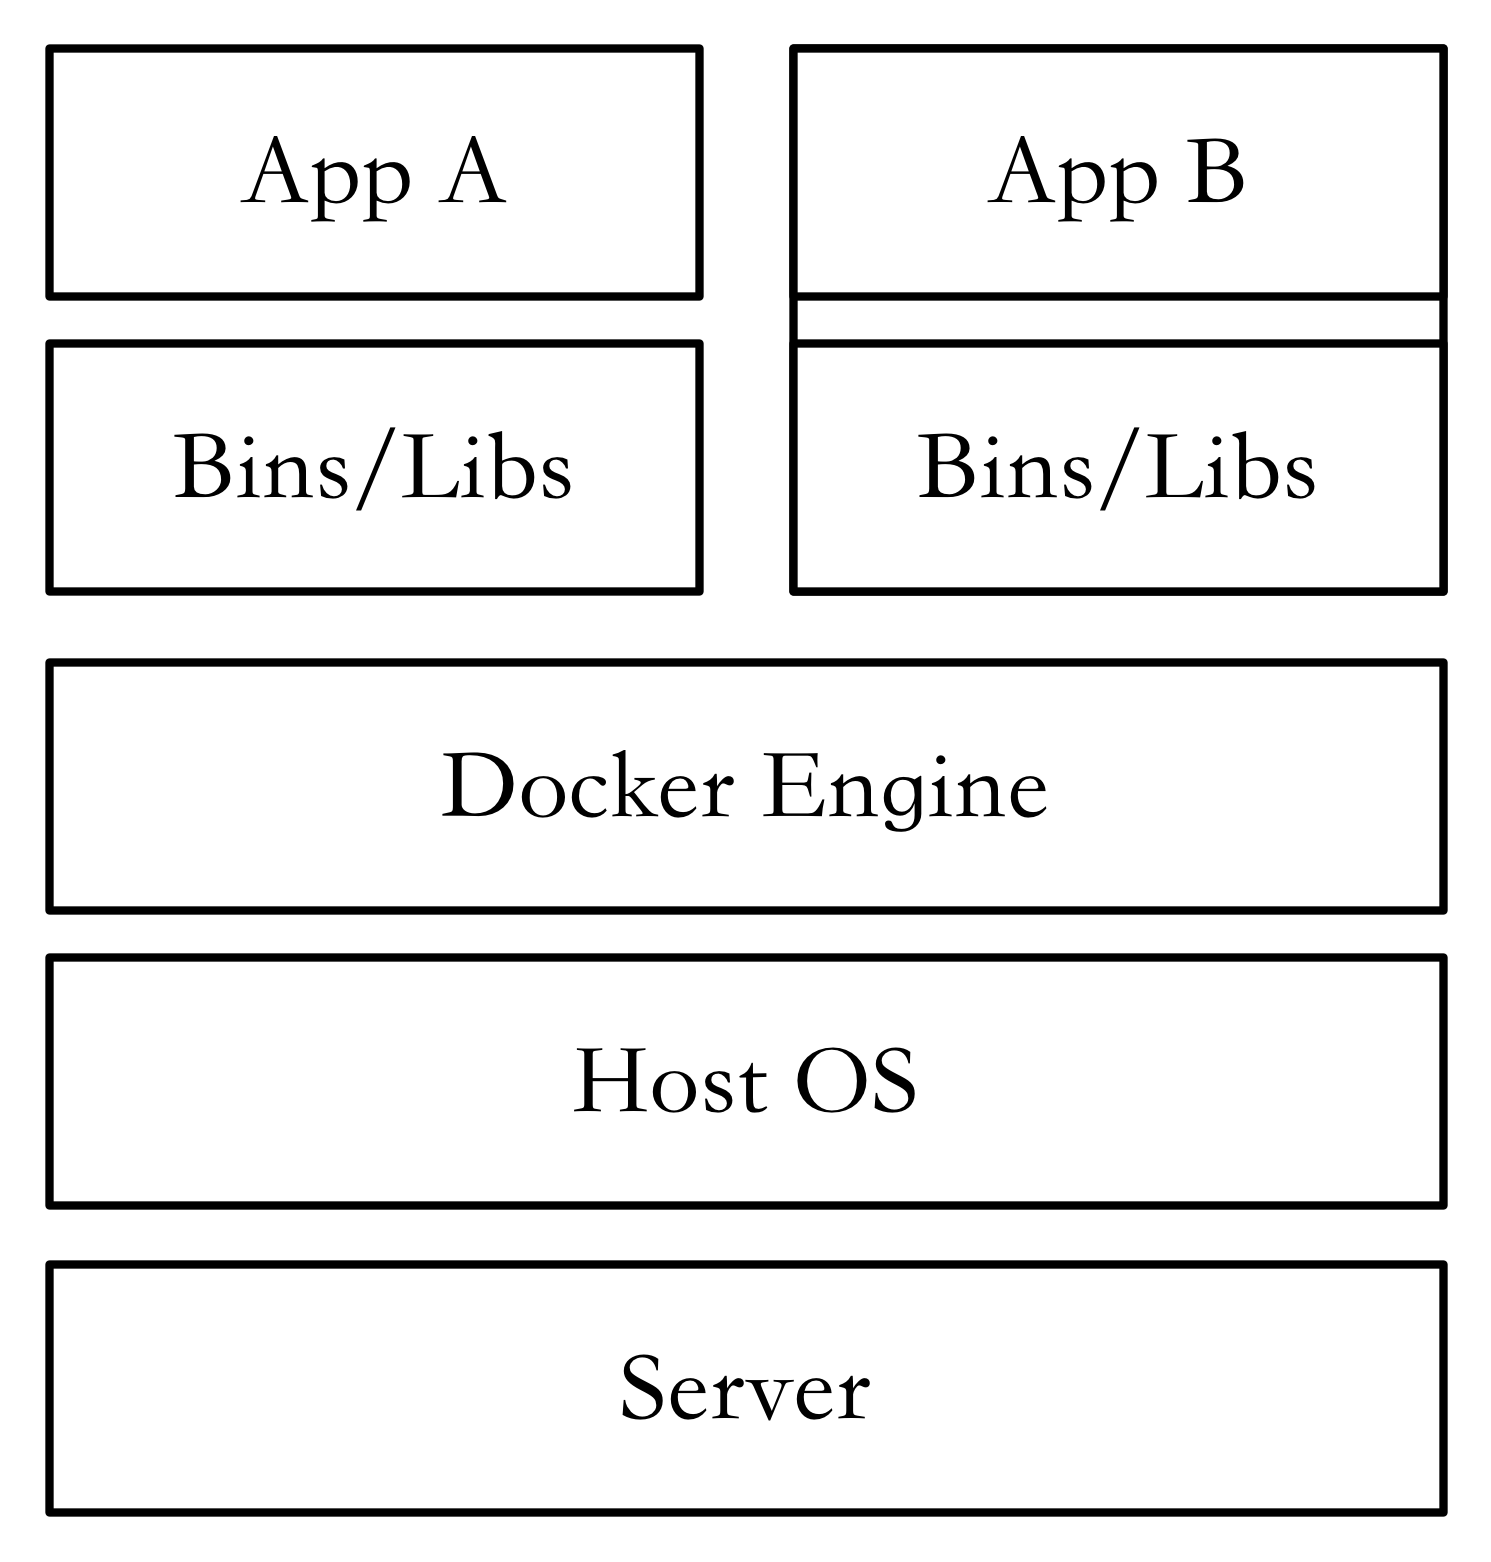
\includegraphics[width=4cm]{./img/02/docker2.png}
      % \caption{docker容器架构}
      \label{fig:docker}
    \end{column}
    \begin{column}{0.50\textwidth}
      \begin{block}{3. 容器化开发部署优化优化}
      同传统虚拟机技术,容器技术的优势包括\cite{chamberlain2014using}:
      \begin{enumerate}
        \item 更高效的利用系统资源
        \item 更快速的启动时间
        \item 一致的运行环境
        \item 更轻松的迁移、维护和扩展
      \end{enumerate}
      \end{block}
    \end{column}
  \end{columns}
  \begin{table}[H]
  \centering
  \begin{minipage}[t]{\linewidth} % 如果想在表格中使用脚注,minipage是个不错的办法
  % \caption[模板文件]{模板文件。如果表格的标题很长,那么在表格索引中就会很不美
  %   观,所以要像 chapter 那样在前面用中括号写一个简短的标题。这个标题会出现在索
  %   引中。}
  \centering
  \caption[Docker]{\scriptsize{同传统虚拟机技术对比}}
  \resizebox{.5\textwidth}{!}{%
  \label{tab:docker-compare}
    \begin{tabularx}{\linewidth}{lXX}
      \toprule[1.5pt]
      {\heiti 对比参数} & {\heiti 容器技术} & {\heiti 虚拟机技术}\\\midrule[1pt]
      启动时间  &  秒级 & 分钟级 \\
      硬盘使用  &  一般为MB  &  一般为GB\\
      应用性能  &  接近原生  &  弱于\\
      系统支持量 & 单机支持上千个容器 & 一般几十个\\
      \bottomrule[1.5pt]
    \end{tabularx}%
  }
  \end{minipage}
\end{table}
\end{frame}


\begin{frame}
\frametitle{二、数据库性能优化}
  \begin{block}{1. InnoDB引擎优化}
  虽然MySQL数据库支持的存储引擎有很多,但是常用的引擎主要是默认的MyISAM和使用最多的InnoDB~\cite{胡雯2012mysql}。
  \end{block}
  \begin{table}[H]
    \centering
    \begin{minipage}[t]{0.8\linewidth} % 如果想在表格中使用脚注,minipage是个不错的办法
    \caption[MySQL]{MySQL数据库存储引擎}
    \scalebox{1.0}[1.0]{%
    \label{tab:mysql-engine}
      \begin{tabularx}{\linewidth}{lX}
        \toprule[1.5pt]
        {\heiti 存储引擎} & {\heiti 描述}\\\midrule[1pt]
        InnoDB  &  支持事务和行级锁,是Mysql上唯一一个提供了外键约束的引擎  \\
        MyISAM  &  基于ISAM存储引擎,常用的引擎,但是不支持事务、行级锁、而且崩溃后不能保证完全恢复。  \\
        \bottomrule[1.5pt]
      \end{tabularx}%
    }
    \end{minipage}
  \end{table}
\end{frame}
\begin{frame}
\frametitle{二、数据库性能优化}
  \begin{block}{1. InnoDB引擎优化}
    \begin{enumerate}
      \item 内存利用方面,调整内存分配以及数据库缓冲池的数量等,保证MySQL在高IO负载时有非常稳定的吞吐~\cite{fruhwirt2010innodb}
      \item IO 控制方面,通过控制线程的并发数和数据的压缩比保证系统正常运行的情况下数据库有更高的效率
      \item 日志控制方面,因为日志文件的大小和实时写入量对于系统的性能来所有很大的影响,在默认情况下,对数据库进行高并发读写,吞吐量在70req/sec左右,优化参数后吞吐量可以提升到300req/sec.
    \end{enumerate}
  \end{block}
\end{frame}
\begin{frame}
\frametitle{二、数据库性能优化}
  \begin{columns}
    \begin{column}{0.50\textwidth}
      \centering
      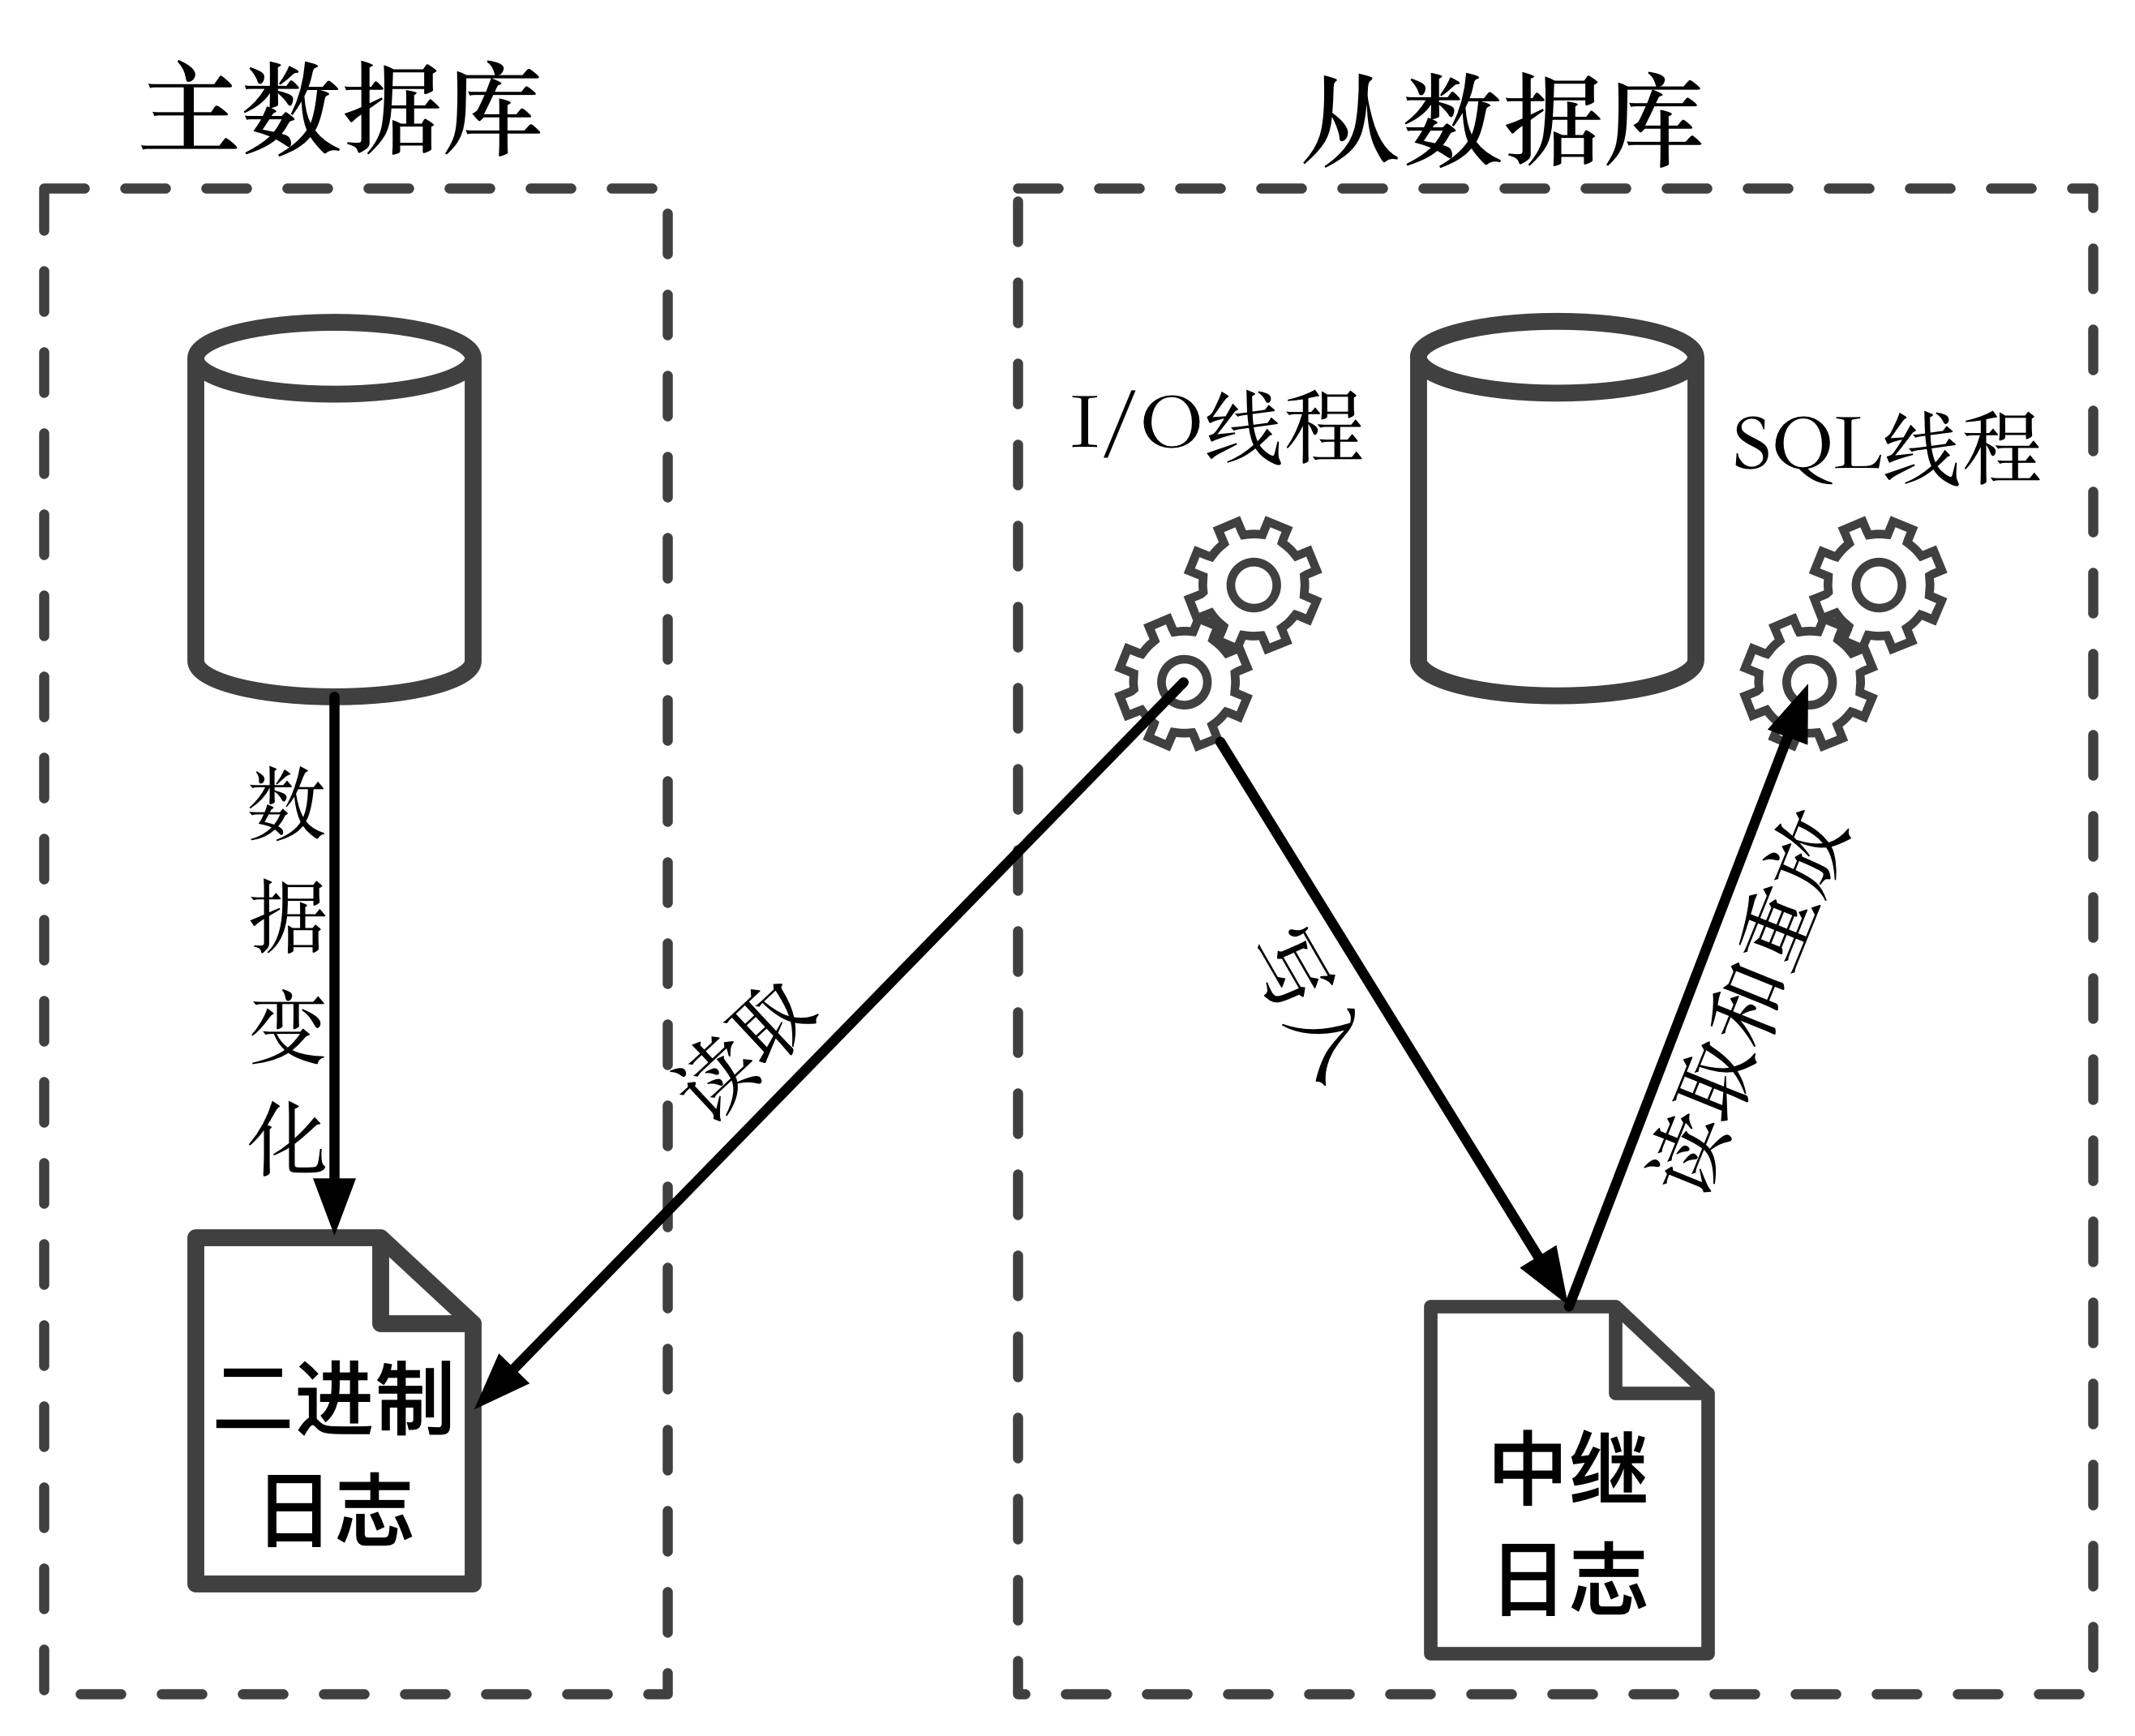
\includegraphics[width=5cm]{./img/03/sql.png}
      % \caption{docker容器架构}
      \label{fig:docker}
    \end{column}
    \begin{column}{0.50\textwidth}
      \begin{block}{2. 数据库复制结构开发}
        开发数据库复制的目的是为了保证当一个节点损坏时,另一个数据库节点能够正常提供服务,当两个节点损坏时,可以通过延时复制的节点以及数据库binlog日志尽可能的恢复平台数据。

        复制的过程主要设计为三步\cite{秦金2013分布式}.
        % \begin{enumerate}
        %   \item 当主数据库的数据发生改变时,主数据库会将数据库数据记录的事务过程写到已经开启的二进制日志文件中;
        %   \item 主库将事务写入二进制文件后会通知从库数据,此时从数据库会链接主数据库将改变的事务日志下载到从数据库的中继日志中;
        %   \item 从数据库对于中继日志中的新事务进行重放,根据日志操作方式修改从数据库的对应数据,保证数据的一致\cite{秦金2013分布式}。
        % \end{enumerate}
      \end{block}
    \end{column}
  \end{columns}
\end{frame}
% \begin{frame}
% \frametitle{二、数据库性能优化}
%   \begin{figure}
%   \centering
%     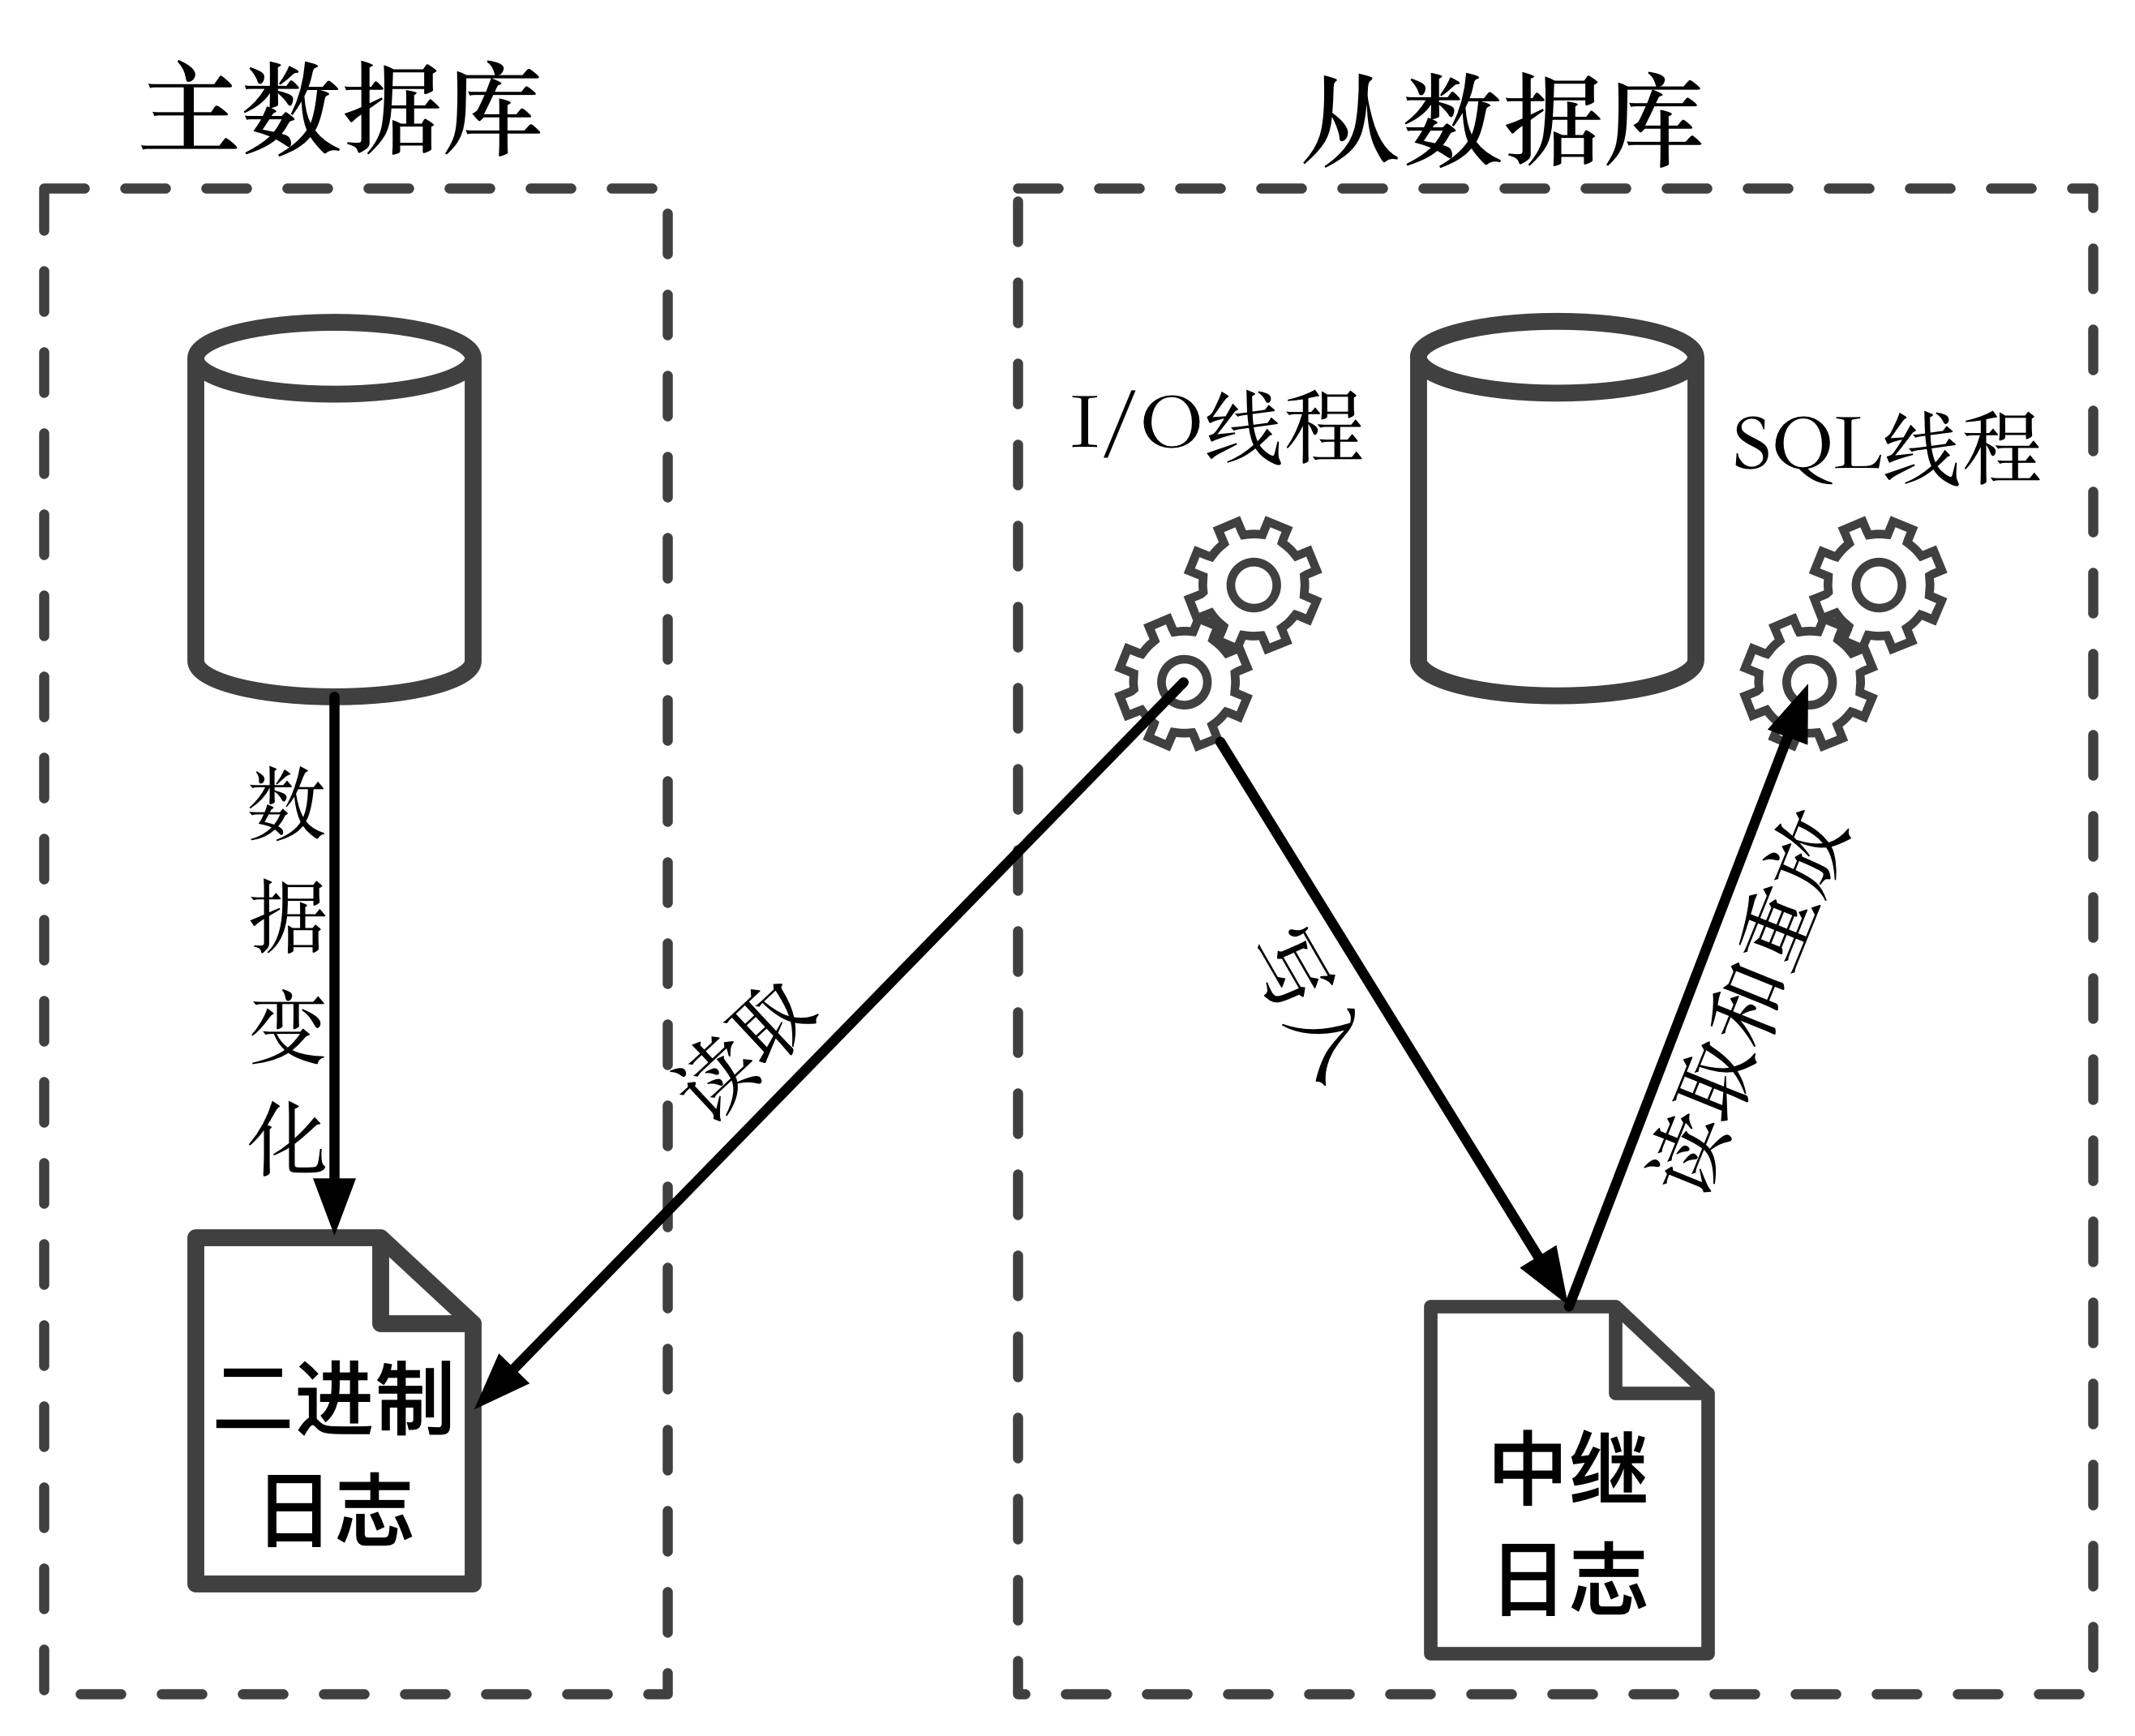
\includegraphics[height=5cm]{./img/03/sql.png}
%     \caption{数据库复制流程}
%     \label{fig:sqlrp}
%   \end{figure}
% \end{frame}


\begin{frame}
\frametitle{三、服务器稳定性优化}
  \begin{block}{1. 应用监控}
    应用监控主要是对Tomcat健康状态的监控,根据监控状态判断自动操作和手动操作,如果是通过重启服务能够解决的异常则会自动的远程重启服务。
    \begin{table}[htb]
      \centering
      \begin{minipage}[t]{0.8\linewidth} % 如果想在表格中使用脚注,minipage是个不错的办法
      \caption[Tomcat]{Tocmat状态}
      \label{tab:tomcat-status}
        \begin{tabularx}{\linewidth}{lX}
          \toprule[1.5pt]
          {\heiti 状态} & {\heiti 描述}\\\midrule[1pt]
          active  &  运行正常  \\
          failed  &  启动失败  \\
          unknown &  未知错误\\
          \bottomrule[1.5pt]
        \end{tabularx}
      \end{minipage}
    \end{table}
  \end{block}
\end{frame}
\begin{frame}
\frametitle{三、服务器稳定性优化}
  为了准确的判断服务异常错误信息,针对服务的不同状态规定不同的状态码,方便运维人员快速判断异常情况。
  \begin{table}[htb]
    \centering
    \begin{minipage}[t]{0.8\linewidth} % 如果想在表格中使用脚注,minipage是个不错的办法
    \caption[Tomcat]{自定义返回状态码}
    \scalebox{0.85}[0.85]{
    \label{tab:tomcat-code}
      \begin{tabularx}{\linewidth}{lX}
        \toprule[1.5pt]
        {\heiti 状态码} & {\heiti 描述}\\\midrule[1pt]
        100  &  表示WEB访问正常  \\
        101  &  表示WEB应用异常,需要查看日志  \\
        102  &  Tomcat服务停止,需要重启  \\
        103  &  服务不存在,需要查看日志\\
        104  &  服务器连接失败,需要查看是网络问题还是服务器异常  \\
        105  &  服务重启  \\
        106  &  其他异常\\
        200  &  重启成功  \\
        201  &  重启失败  \\
        \bottomrule[1.5pt]
      \end{tabularx}
      }
    \end{minipage}
  \end{table}
\end{frame}
\begin{frame}
\frametitle{三、服务器稳定性优化}
  通过开发监控和重启的python脚本以及短信通知的python脚本实现具体操作,通过shell调用脚本实现日志记录和其他扩展。
  \begin{figure}
  \centering
    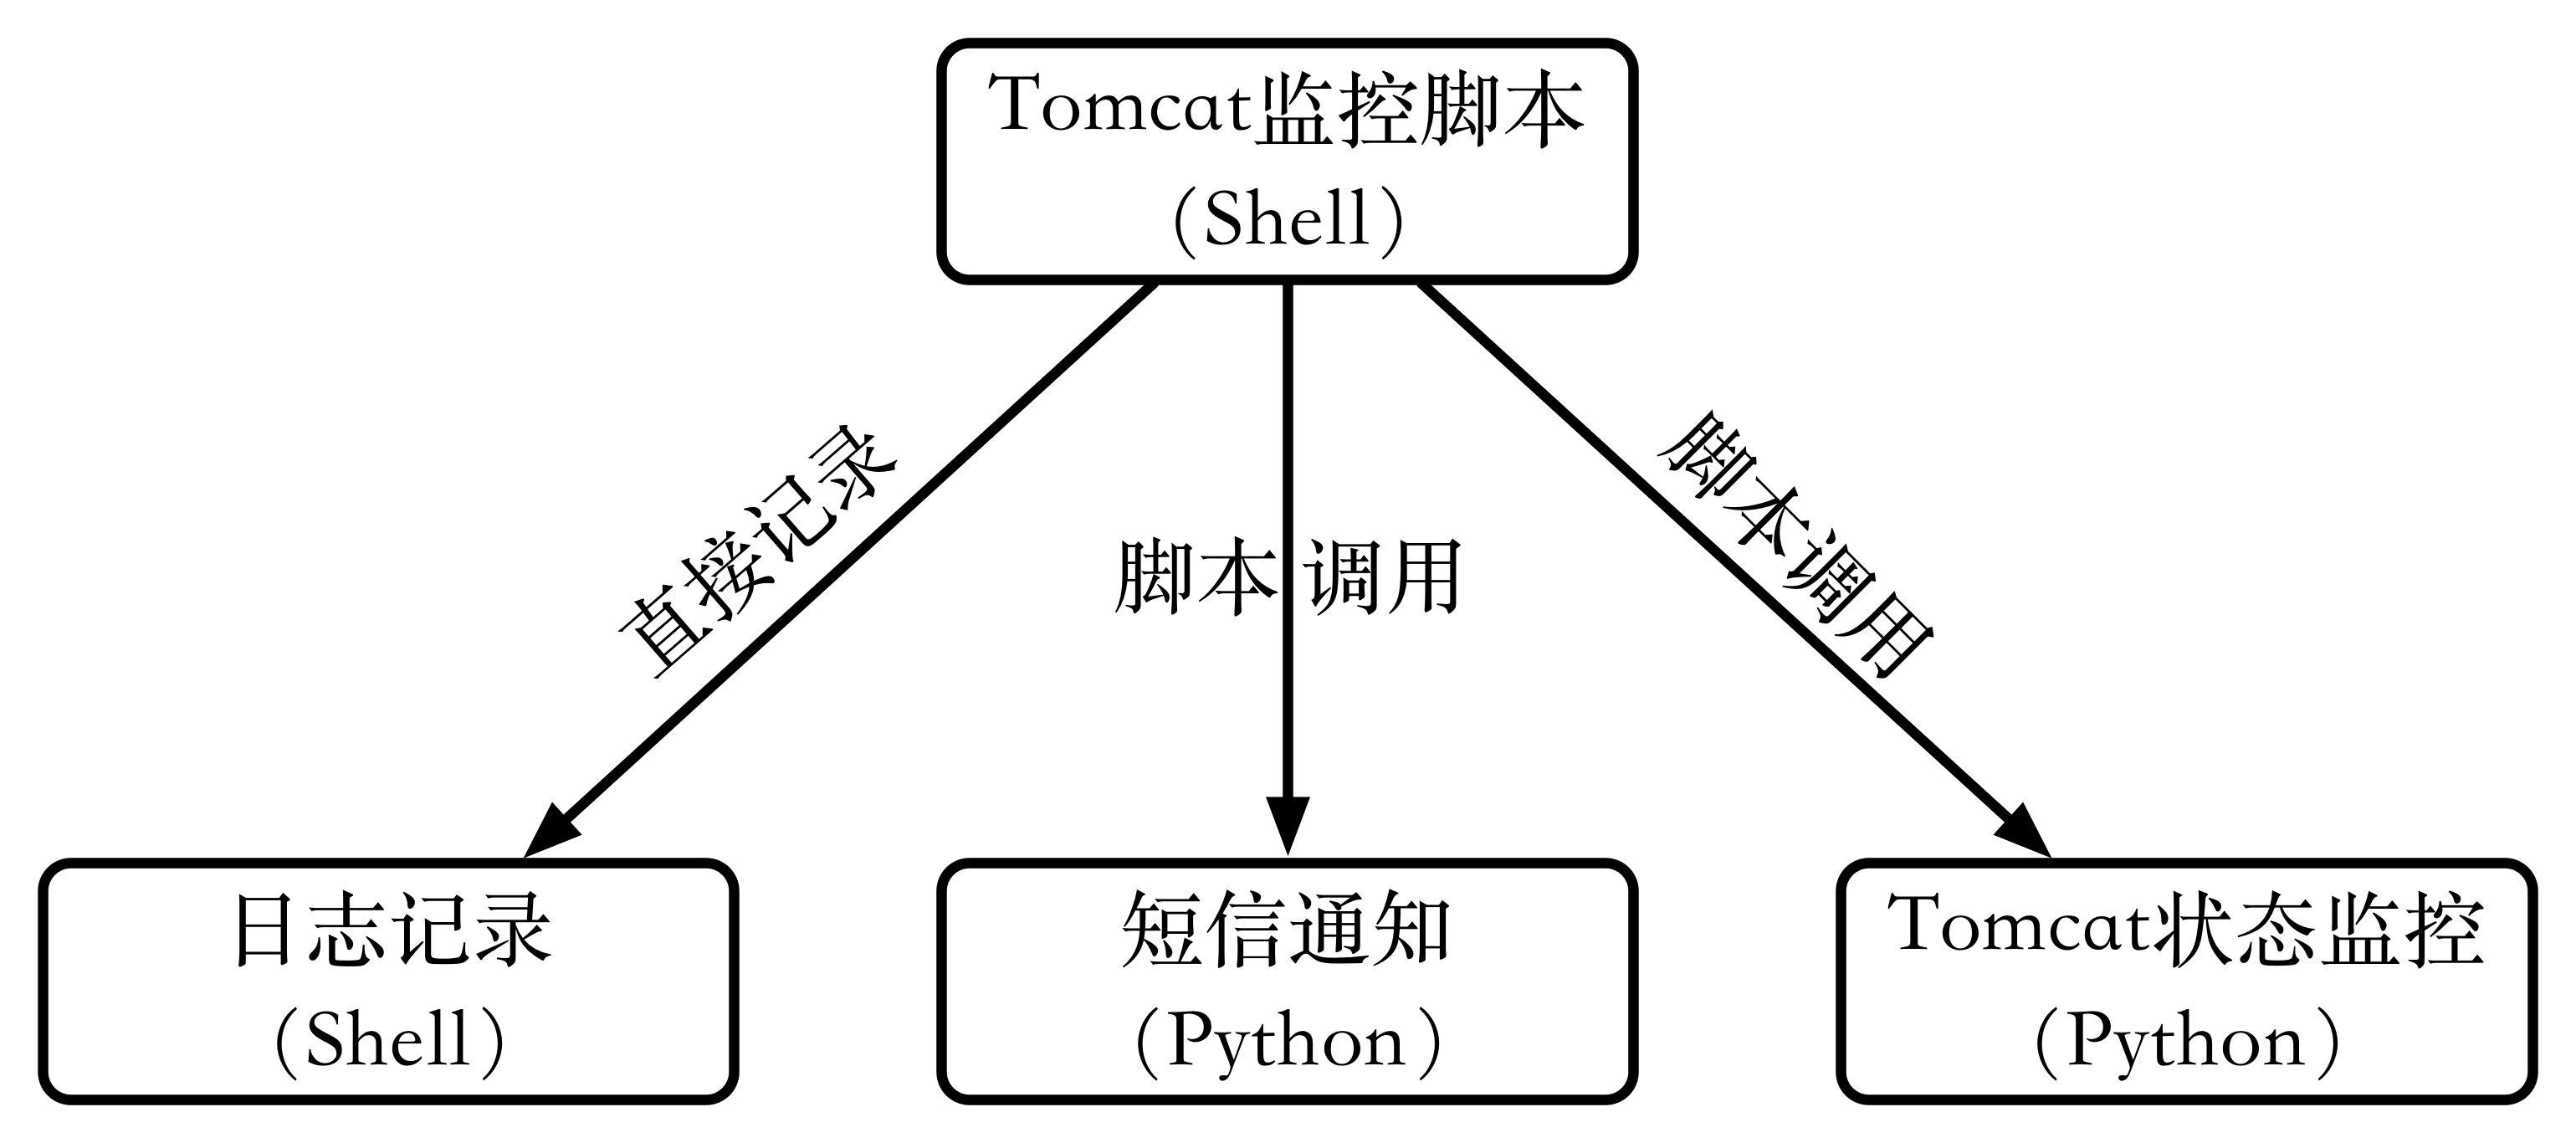
\includegraphics[height=4cm]{./img/03/tomcat2.png}
    \caption{tomcat监控框架}
    \label{fig:tomcat}
  \end{figure}
\end{frame}
\begin{frame}
\frametitle{三、服务器稳定性优化}
  \begin{block}{2. 数据健康监控}
    \begin{itemize}
      \item \footnotesize{为了保证数据库的正常运行,通过开发shell脚本实现mysql的服务状态监控,当一个节点出现异常时,会通过API动态调整阿里云数据库负载均衡的权重,保证正常的节点能持续提供服务,同时对异常节点进行恢复处理。}
    \end{itemize}
  \end{block}
  \begin{figure}
  \centering
    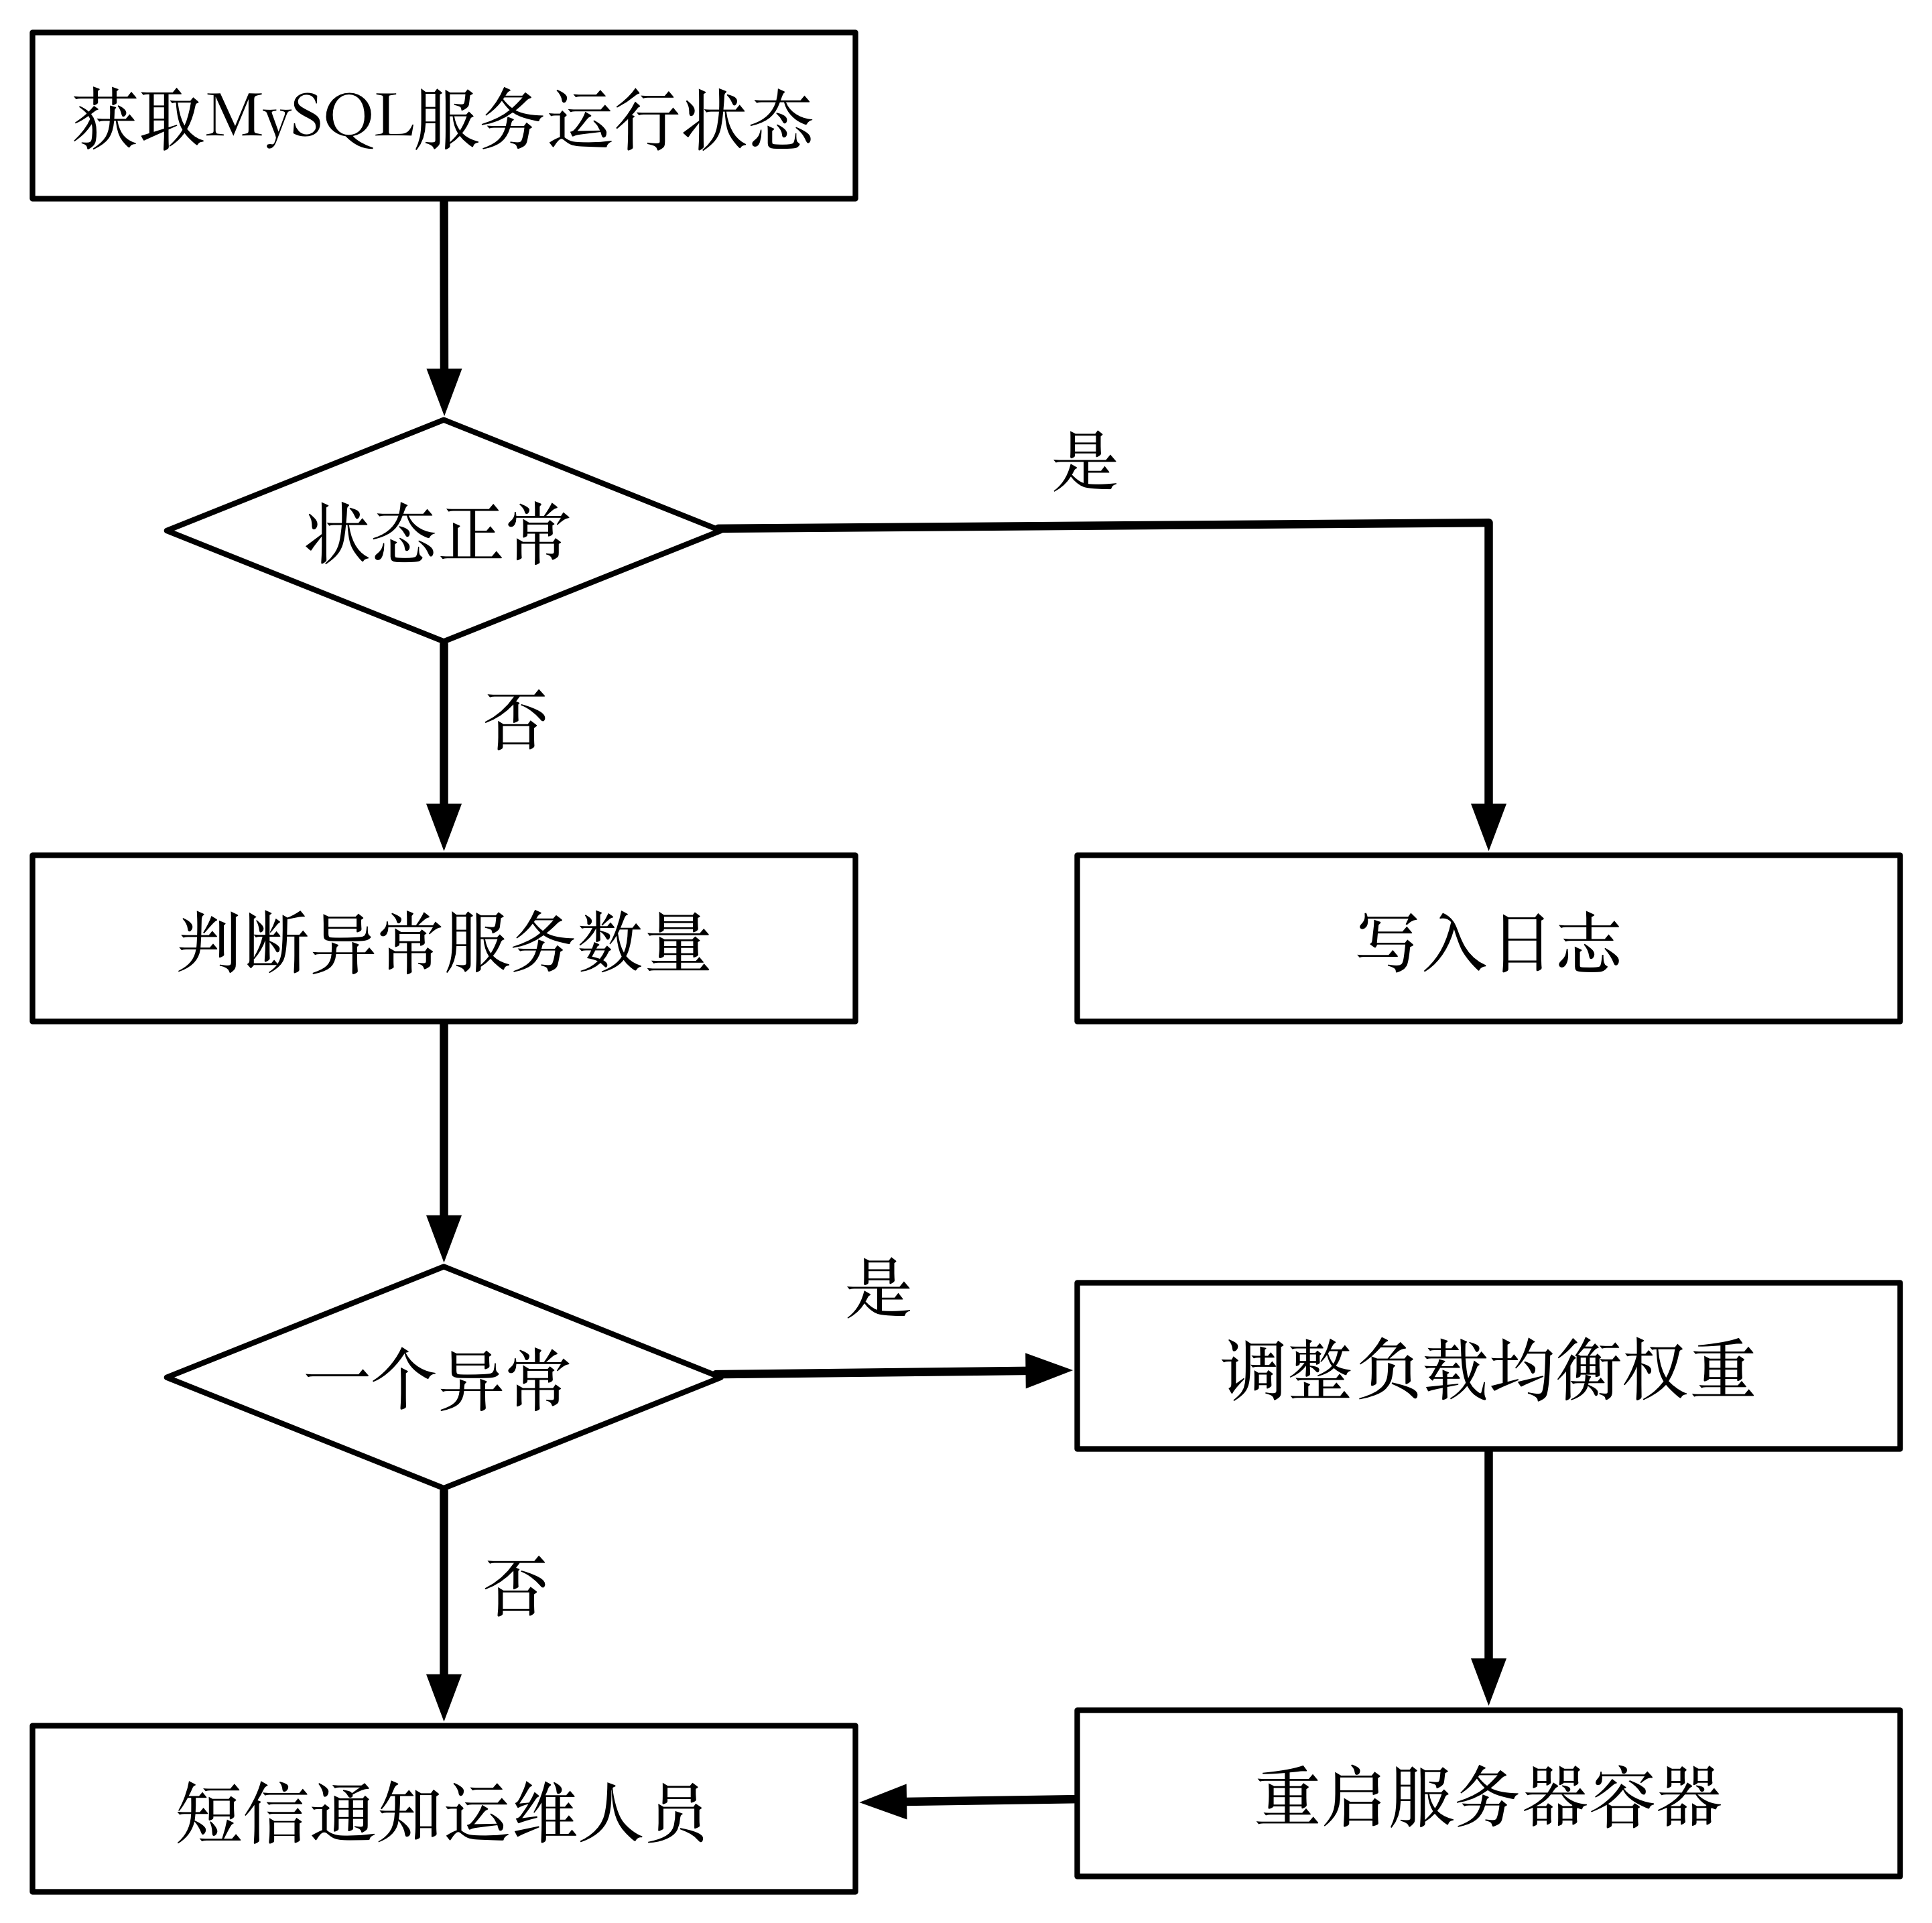
\includegraphics[height=4cm]{./img/03/mysql1.png}
    \caption{mysql健康监控}
    \label{fig:mysql1}
  \end{figure}
\end{frame}
\begin{frame}
\frametitle{三、服务器稳定性优化}
  \begin{block}{2. 数据同步监控}
    \begin{itemize}
      \item \footnotesize{因为两个数据库节点进行双主复制,当一个损坏时另外一个提供服务,这就要求两个数据库的内容保持一致,因此需要实时监控数据库的同步状态,保证两个库的数据一致。}
    \end{itemize}
  \end{block}
  \begin{figure}
  \centering
    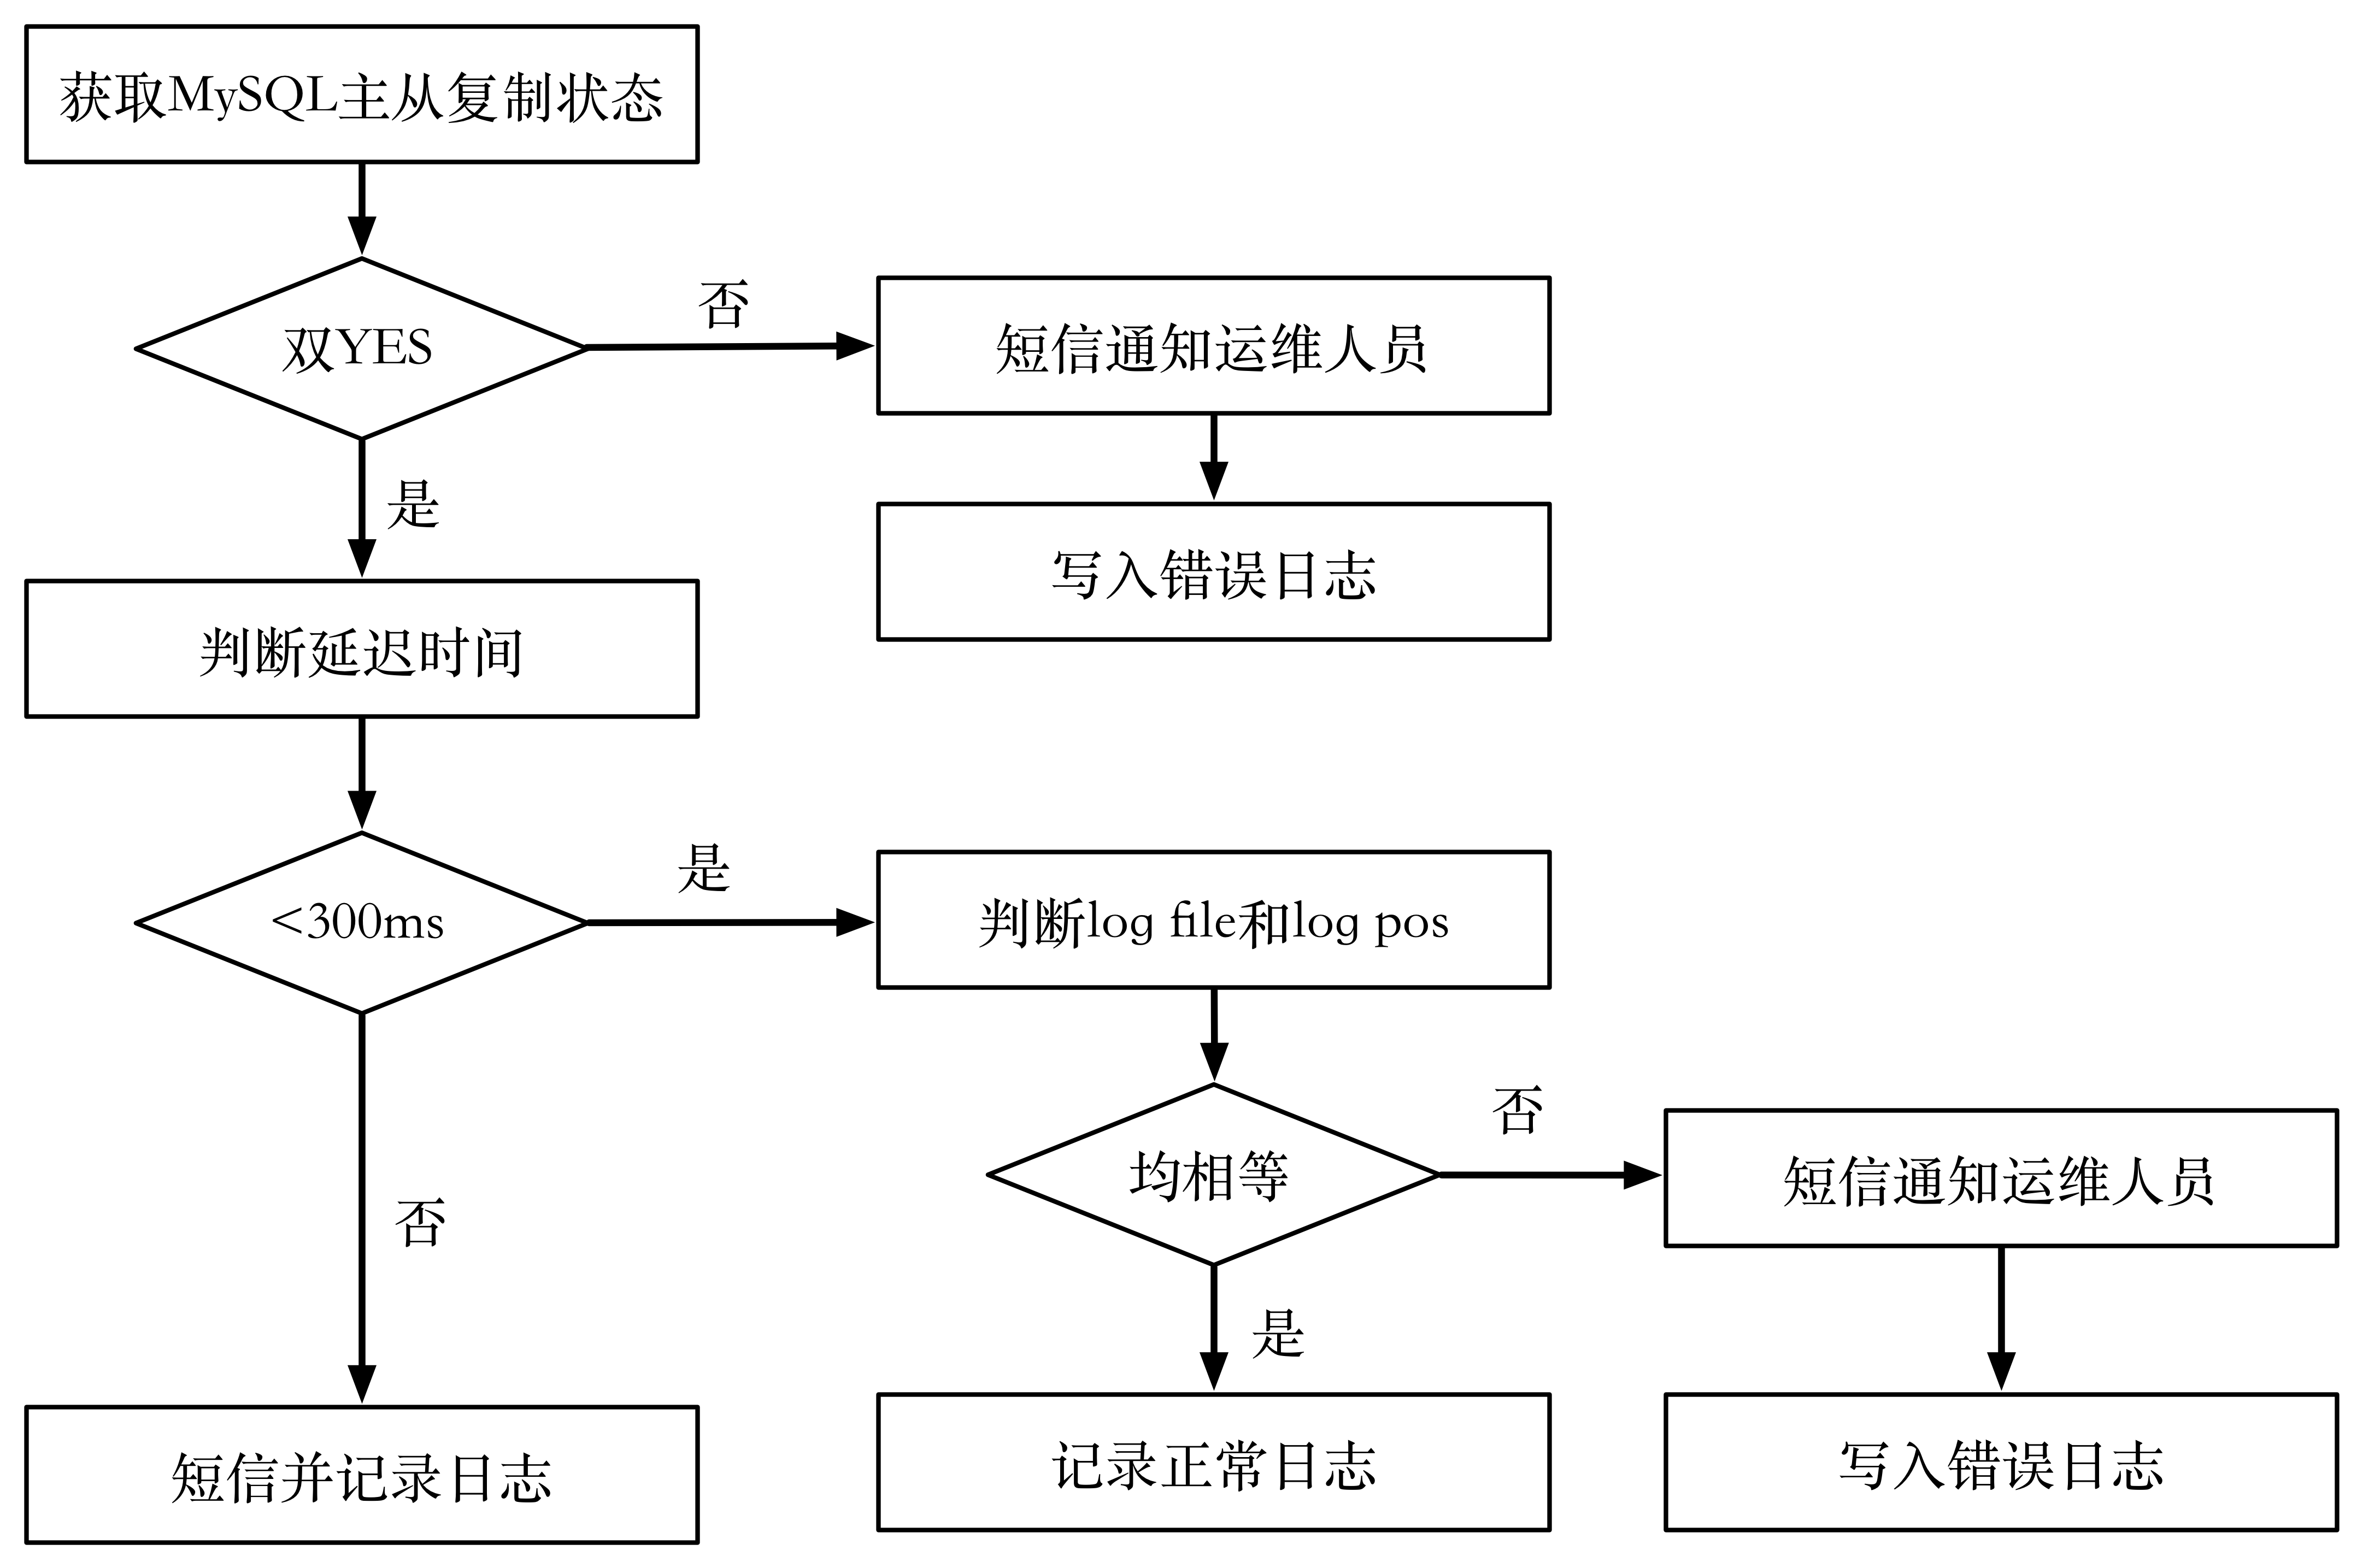
\includegraphics[height=4cm]{./img/03/mysql2.png}
    \caption{mysql同步监控}
    \label{fig:mysql2}
  \end{figure}
\end{frame}
\begin{frame}
\frametitle{三、服务器稳定性优化}
  \begin{block}{3. 心跳监听开发}
    \begin{figure}
    \centering
      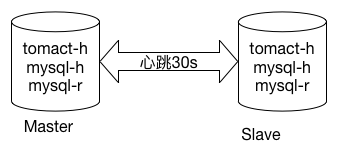
\includegraphics[height=3cm]{./img/03/ha.png}
      \caption{心跳监听模型}
      \label{fig:mysql2}
    \end{figure}
    Heartbeat 是一款开源的提供高可用(Highly-Available)服务的软件,通过 Heart- beat 可以将资源(IP 及程序服务等资源)从一台已经故障的计算机快速转移到另一 台正常运转的机器上继续提供服务,称之为高可用服务~\cite{郭绪晶2012服务器集群系统高可用模块设计与实现}。
  \end{block}
\end{frame}
\begin{frame}
\frametitle{三、服务器稳定性优化}
  \begin{block}{4. 通知和备份方案设计}
    \begin{itemize}
      \item 在第一时间通知运维人员服务器状态,开发短信通知脚本;
      \item 对异常进行细致的分析,准确定位异常原因,需要对所有的监控程序进行日志的保存和备份。
    \end{itemize}
  \end{block}
  \begin{columns}
    \begin{column}{0.30\textwidth}
      \centering
      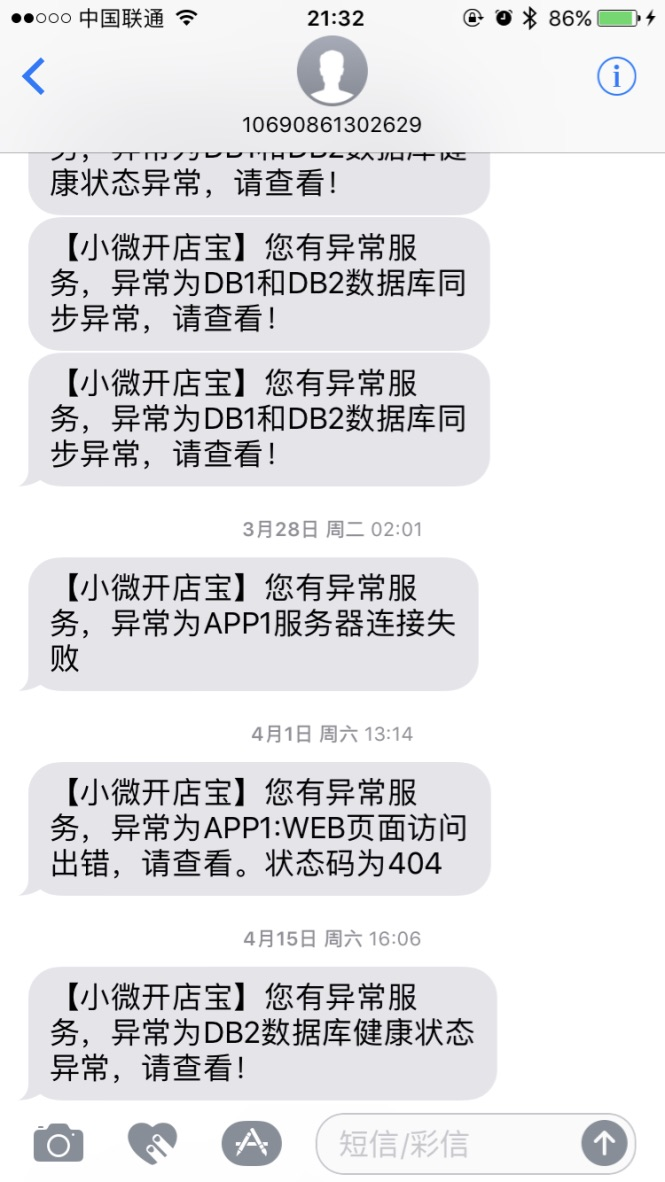
\includegraphics[width=2cm]{./img/03/message.jpg}
    \end{column}
    \begin{column}{0.70\textwidth}
      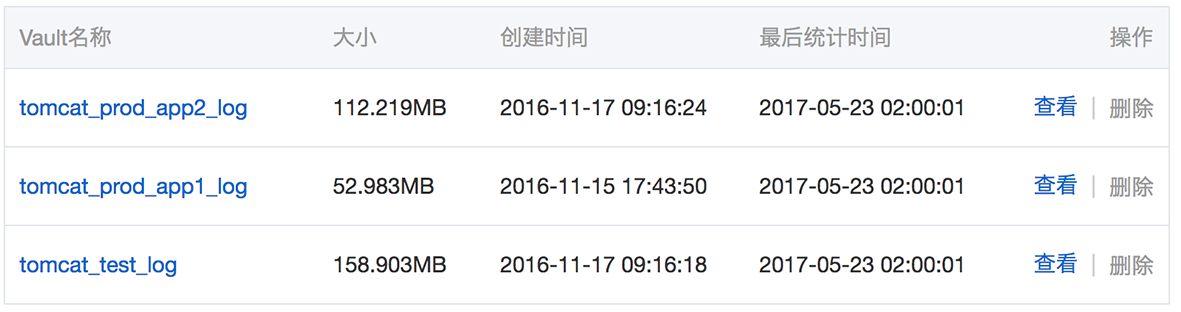
\includegraphics[width=7cm]{./img/03/aliyun3.png}
    \end{column}
  \end{columns}
\end{frame}

%% ++++++++++++++++++++++++++++++++++++++++++++++++++++++
%%      研究方案
%% ++++++++++++++++++++++++++++++++++++++++++++++++++++++
\begin{frame}
  \frametitle{结论及展望}
  \begin{block}{总结}
    通过应用、数据和服务器三个层级的优化策略研究,目前应用服务较优化前相比,单个服务器的负载达到了比较好的程度,应用的访问速度提升了接近20\%, 新版的部署时间节省了50\%。
  \end{block}
  \begin{block}{展望}
  虽然通过本论文的优化,WEB 应用的性能得到了较大的提升,但是目前的 WEB 应用系统依然有很大的改进空间:
    \begin{enumerate}
      \item 探索数据库读写分离方案,从数据库的输入输出两个方面进行优化,更好的保证数据的完整性;
      \item 探索基于kubernetes的容器化集群部署方案以及监控方案;
    \end{enumerate}
  \end{block}
\end{frame}


%% ++++++++++++++++++++++++++++++++++++++++++++++++++++++
%%      进展情况
%% ++++++++++++++++++++++++++++++++++++++++++++++++++++++
% \begin{frame}
% \frametitle{后续工作安排}
%   \begin{block}{已完成 }
% 	\begin{itemize}
% 		\item 平台功能开发
% 		\item Jenkins自动化测试、部署工具的配置和部署脚本开发
%         		\item Couchbase缓存机制的开发
% 		\item ElasticSearch分布式全文搜索引擎的部署和测试
% 	\end{itemize}
%   \end{block}
%   \begin{block}{进行中}
% 	\begin{itemize}
%     \item 缓存和搜索接口的开发
%     \item 推荐系统的开发
% 	\end{itemize}
%   \end{block}
% \end{frame}

%% ++++++++++++++++++++++++++++++++++++++++++++++++++++++
%%      Last Page
%% ++++++++++++++++++++++++++++++++++++++++++++++++++++++
% \begin{frame}
% \frametitle{大学生创业平台的开发与系统优化策略研究}
%   谢谢各位老师的聆听!
% \end{frame}

%% ++++++++++++++++++++++++++++++++++++++++++++++++++++++
%%      Reference Page
%% ++++++++++++++++++++++++++++++++++++++++++++++++++++++
\begin{frame}[allowframebreaks]{References}
  \scriptsize
  \bibliographystyle{plain}
  \bibliography{myRefs}
\end{frame}

\end{document}
%% ======================================================
